\documentclass{ieeeaccess}
\usepackage[utf8]{inputenc}
\usepackage[T1]{fontenc}
\usepackage{cite}
\usepackage{amsmath,amssymb,amsfonts}
\usepackage{graphicx}
\usepackage{textcomp}
\usepackage{booktabs}
\usepackage{makecell}
\usepackage{url}
\usepackage{microtype}
\usepackage{float}

\newdimen\xfigwd
\xfigwd=\columnwidth

\def\BibTeX{{\rm B\kern-.05em{\sc i\kern-.025em b}\kern-.08em
    T\kern-.1667em\lower.7ex\hbox{E}\kern-.125emX}}

\begin{document}
\history{Date of publication xxxx 00, 0000, date of current version xxxx 00, 0000.}
\doi{xxx}

\title{Integración de Blockchain para la Trazabilidad y Auditoría en el Entrenamiento Distribuido de Modelos de Inteligencia Artificial}

\author{\uppercase{David Piotr Znojek}\authorrefmark{1}, and
\uppercase{Francisco A. Pujol}\authorrefmark{1}, \IEEEmembership{Senior Member, IEEE}}

\address[1]{Departamento de Tecnología Informática y Computación, Escuela Politécnica Superior, Universidad de Alicante, 03690 San Vicente del Raspeig, Alicante, España (e-mail: dawidznojek@gmail.com, fpujol@ua.es)}
\tfootnote{}

\markboth
{D. P. Znojek and F. A. Pujol: Integración de Blockchain para Trazabilidad y Auditoría en Aprendizaje Federado}
{D. P. Znojek and F. A. Pujol: Integración de Blockchain para Trazabilidad y Auditoría en Aprendizaje Federado}

\corresp{Corresponding author: David Piotr Znojek (e-mail: dawidznojek@gmail.com).}

\begin{abstract}
El entrenamiento distribuido mediante Aprendizaje Federado (\textit{Federated Learning}) permite preservar la privacidad de datos sensibles pero carece intrínsecamente de mecanismos para auditar la legitimidad de las contribuciones de los participantes, exponiendo al sistema a ataques de envenenamiento (\textit{model poisoning}) con consecuencias críticas en sectores como el de los vehículos autónomos. En este artículo se presenta y evalúa una arquitectura híbrida que integra una red Blockchain permisionada basada en Hyperledger Besu y consenso IBFT 2.0 con el framework Flower y almacenamiento distribuido fuera de cadena mediante IPFS. Se diseña un contrato inteligente en Solidity que implementa un protocolo de doble verificación cruzada entre clientes y servidor agregador utilizando compromisos criptográficos SHA-256 de los pesos neuronales. La viabilidad del marco se valida empíricamente sobre un banco de pruebas distribuido entrenando un clasificador convolucional de señales y eventos viales bajo un riguroso protocolo experimental multiejecución (15 ejecuciones y 450 rondas federadas en total) bajo cinco configuraciones. Los resultados cuantitativos demuestran que, en el despliegue distribuido realista, la capa de trazabilidad añade una sobrecarga temporal reducida de tan solo el 9,5\% (6,34~s por ronda), manteniendo un coste de gas estable y predecible por transacción y escalando con un impacto marginal (+0,39~s en mediana de ronda y +0,10~s en confirmación de bloque) al ampliar el quórum de 4 a 7 nodos validadores ($f=1 \to f=2$). Asimismo, la evaluación adversarial valida funcionalmente la intercepción determinista de manipulaciones en tránsito y contribuciones desalineadas tanto en servidor como en clientes con latencias de mitigación en tornno a 0,10~s (149~ms para aborto local preventivo y 31~ms para descarte en agregación). Esta investigación confirma que el coste de incorporar inmutabilidad y no repudio resulta plenamente asumible frente a las garantías de auditoría obtenidas.
\end{abstract}

\begin{keywords}
Aprendizaje Federado, Auditoría Criptográfica, Blockchain, Consenso IBFT 2.0, Hyperledger Besu, IPFS, Trazabilidad, Vehículos Autónomos.
\end{keywords}

\titlepgskip=-15pt

\maketitle

% !TeX root = ../main.tex
\section{Introducción}
\label{sec:introduccion}

\PARstart{E}{l} auge de la Inteligencia Artificial (IA) y del Aprendizaje Automático (\textit{Machine Learning}, ML) ha transformado sectores críticos como la salud, las finanzas y la conducción autónoma. No obstante, el entrenamiento de modelos de gran capacidad requiere volúmenes masivos de datos, frecuentemente sensibles o confidenciales (geolocalización, hábitos de consumo o registros biométricos). En los paradigmas tradicionales centralizados, la recopilación de información en un único repositorio introduce graves riesgos de privacidad, problemas de cumplimiento normativo (como el RGPD) y cuellos de botella computacionales y energéticos.

El Aprendizaje Federado (\textit{Federated Learning}, FL)~\cite{mcmahan2017federated} surgió como una alternativa descentralizada en la que múltiples nodos o clientes entrenan copias locales del modelo con sus propios datos privados, transmitiendo a un servidor central únicamente los parámetros o gradientes actualizados. Aunque FL solventa en gran medida la fuga de datos crudos, introduce una vulnerabilidad estructural: la falta de confianza intrínseca entre los participantes. En un entorno distribuido no supervisado, actores maliciosos o nodos comprometidos pueden ejecutar ataques de envenenamiento (\textit{data poisoning} o \textit{model poisoning}) e inserción de puertas traseras (\textit{backdoors})~\cite{bagdasaryan2020backdoor} inyectando pesos manipulados. Por ejemplo, en el contexto de los Vehículos Conectados y Autónomos (CAV)~\cite{chellapandi2024federated}, una pequeña alteración coordinada en los pesos podría inducir al modelo global a no clasificar correctamente una señal de tráfico crítica (como un STOP), con consecuencias potencialmente fatales.

Para mitigar este riesgo, la integración de la tecnología \textit{Blockchain} con Aprendizaje Federado (BCFL)~\cite{qu2022blockchain} ofrece una solución idónea como registro contable inmutable, descentralizado y verificable~\cite{nakamoto2008bitcoin, zheng2018blockchain}. Al integrar Blockchain en un flujo de entrenamiento distribuido, cada actualización de parámetros, ronda de agregación e identidad de los clientes queda registrada criptográficamente mediante contratos inteligentes (\textit{smart contracts}), habilitando una trazabilidad integral, verificable y no repudiable de las contribuciones.

Sin embargo, esta convergencia plantea un compromiso técnico fundamental: el dilema entre \textbf{seguridad y rendimiento}. Mientras que la Blockchain aporta inmutabilidad y consenso tolerante a fallos bizantinos, introduce una sobrecarga inevitable de latencia de red, tiempo de confirmación de transacciones y consumo de recursos. En aplicaciones vehiculares de misión crítica o en tiempo cuasi-real en el borde (\textit{edge computing})~\cite{liu2019edge}, resulta imperativo responder a la siguiente pregunta: \textit{¿cuánta latencia y coste computacional estamos dispuestos a asumir a cambio de un entrenamiento auditable y más resistente a manipulaciones?}

\subsection{Motivación y Trabajos Previos}
Este trabajo se fundamenta y amplía dos líneas de investigación desarrolladas en la Universidad de Alicante:
\begin{enumerate}
    \item \textbf{Verificación de eventos vehiculares en tiempo real}~\cite{pujol2024blockchain}: demostró la viabilidad de una red privada Hyperledger Besu con consenso IBFT 2.0 para registrar alertas de tráfico con latencias de 0,32 a 0,82 segundos, mejorando el tiempo de respuesta humano.
    \item \textbf{Framework FL-Blockchain}~\cite{cloudlabaia_flblockchain}: planteó conceptualmente el uso de contratos inteligentes para registrar los \textit{hashes} criptográficos de los pesos de entrenamiento en cada ronda federada.
\end{enumerate}

La presente investigación valida, formaliza e implementa experimentalmente la convergencia de ambas propuestas en un banco de pruebas real, evaluando tanto la integridad como el impacto en el rendimiento temporal.

\subsection{Contribuciones Principales}
Las contribuciones de este artículo se resumen en los siguientes puntos:
\begin{itemize}
    \item \textbf{Diseño de una arquitectura híbrida}: Se formula un marco integral que acopla una red permisionada basada en Hyperledger Besu con el framework de aprendizaje federado Flower~\cite{beutel2020flower} y un sistema de almacenamiento distribuido direccionable por contenido (IPFS).
    \item \textbf{Trazabilidad e integridad mediante Smart Contracts}: Se diseña un contrato inteligente en Solidity que orquesta la verificación cruzada de modelos mediante resúmenes SHA-256, registrando de forma inalterable las contribuciones de cada cliente y el modelo global consolidado por ronda.
    \item \textbf{Evaluación empírica y mitigación de ataques adversariales}: Se somete la infraestructura a vectores de ataque deliberados de inyección de pesos corruptos (tanto en servidor comprometido como en clientes envenenadores), validando la capacidad del protocolo de doble verificación para detectar y neutralizar de forma determinista cualquier discrepancia de integridad o modelo no registrado on-chain (alcanzando una tasa de éxito del 100\% en los vectores de adulteración evaluados) con tiempos de reacción inferiores a $0{,}1$~segundos.
    \item \textbf{Evaluación cuantitativa de la infraestructura}: Se despliega un clasificador convolucional de tráfico con el propósito de emplear la estructura de aprendizaje federado como banco de pruebas experimental para extraer métricas cuantitativas reproducibles (sobrecoste temporal, consumo de gas y escalabilidad de validadores), delimitando la optimización fina del modelo como trabajo futuro.
    \item \textbf{Análisis de viabilidad operativa}: Se responde analíticamente al dilema latencia-seguridad, delimitando los escenarios en los que la sobrecarga del registro en cadena resulta plenamente asumible frente a esquemas no auditables.
\end{itemize}

Con el fin de facilitar la reproducibilidad y la transferencia científica, el código fuente completo del framework, los contratos inteligentes en Solidity, las plantillas de despliegue de la red Hyperledger Besu con Docker Compose y los scripts de experimentación se encuentran publicados de forma abierta en el repositorio de GitHub: \url{https://github.com/dpz6-ua/Blockchain_ML}.

\subsection{Estructura del Artículo}
El resto del manuscrito se estructura de la siguiente manera: la Sección~\ref{sec:estado_arte} expone el estado del arte y fundamentos teóricos de Blockchain y Aprendizaje Federado. La Sección~\ref{sec:arquitectura} detalla la arquitectura propuesta y el diseño del contrato inteligente. La Sección~\ref{sec:implementacion} describe el banco de pruebas experimental y el dataset empleado. La Sección~\ref{sec:evaluacion} presenta y discute los resultados de rendimiento y seguridad. Finalmente, la Sección~\ref{sec:conclusiones} resume las conclusiones y líneas futuras.


% !TeX root = ../main.tex
\section{Fundamentos Teóricos y Trabajos Relacionados}
\label{sec:estado_arte}

La arquitectura propuesta converge tres pilares tecnológicos: registros distribuidos permisionados con consenso BFT, almacenamiento direccionable por contenido y aprendizaje federado. A continuación se sintetizan sus fundamentos teóricos y las limitaciones detectadas en la literatura.

\subsection{Blockchain Permisionada y Consenso IBFT 2.0}
Una cadena de bloques es una estructura de datos inmutable y distribuida en la que las transacciones se agrupan en bloques encadenados mediante funciones hash criptográficas resistentes a colisiones (como SHA-256)~\cite{nist2015sha, zheng2018blockchain}. Frente a las redes públicas (\textit{permissionless}) como Bitcoin o Ethereum Mainnet, penalizadas por altas latencias y costes económicos de transacción, los consorcios industriales adoptan redes permisionadas basadas en la Máquina Virtual de Ethereum (EVM)~\cite{buterin2014ethereum}, tales como Hyperledger Besu~\cite{besu_docs}.

En estos entornos, los mecanismos basados en consumo de recursos (PoW) o capital (PoS) se sustituyen por algoritmos de tolerancia a fallos bizantinos. El protocolo \textbf{IBFT 2.0} (\textit{Istanbul Byzantine Fault Tolerant})~\cite{moniz2020istanbul} estructura el consenso en torno a un conjunto predefinido de validadores que alternan el rol de proponente mediante un esquema rotatorio (\textit{round-robin}). Un bloque solo se anexa a la cadena tras una votación en tres fases (pre-prepare, prepare, commit) firmada por una supermayoría de al menos dos tercios:
\begin{equation}
n \ge 3f + 1
\end{equation}
donde $n$ denota el número total de nodos validadores y $f$ el número máximo de participantes defectuosos o bizantinos tolerables. 

IBFT 2.0 ofrece una propiedad determinante frente a otros consensos: la \textbf{finalidad determinista inmediata}. Al carecer de bifurcaciones probabilísticas (\textit{forks}), una vez que una ronda de entrenamiento o contribución se sella en un bloque, adquiere finalidad inmediata e inmutabilidad en el libro mayor distribuido. Asimismo, aunque el precio del gas (\textit{gas price}) se configure en cero para anular tarifas monetarias, el cómputo de \textit{gas used}~\cite{ethereum_gas} se mantiene como métrica objetiva del coste de cómputo y almacenamiento impuesto a la red.

\subsection{Almacenamiento Distribuido Off-Chain (IPFS)}
El almacenamiento directo de redes neuronales profundas en una Blockchain es inviable debido al tamaño de los pesos (decenas o cientos de megabytes), lo cual provocaría una saturación crítica del estado de la EVM (\textit{state bloat}) y un consumo prohibitivo de gas.

Para superar este cuello de botella, se implementa el paradigma de \textbf{almacenamiento fuera de cadena con compromiso dentro de cadena} (\textit{off-chain storage with on-chain commitment}) utilizando el Sistema de Archivos Interplanetario (IPFS)~\cite{benet2014ipfs, daniel2022ipfs}. IPFS opera sobre una topología P2P basada en direccionamiento por contenido (\textit{content addressing}) y estructuras de grafo acíclico dirigido (Merkle DAG)~\cite{daniel2022ipfs, trautwein2022design}: cada archivo se fragmenta en bloques inmutables y se identifica de forma unívoca mediante un \textit{Content Identifier} (CID), obtenido a partir del hash criptográfico de su contenido. La rigurosa evaluación arquitectural y empírica de IPFS a escala global realizada por Trautwein et al.~\cite{trautwein2022design} demuestra que su protocolo de intercambio de bloques (Bitswap) y la tabla hash distribuida (Kademlia DHT) posibilitan transferencias descentralizadas con baja sobrecarga de enrutamiento. Al desacoplar el almacenamiento de pesos neuronales en IPFS y registrar únicamente el identificador de contenido (CIDv0 de IPFS, que encapsula el multihash SHA-256 del artefacto serializado) en el contrato inteligente~\cite{zhao2021privacy}, se asegura que cualquier descarga posterior sea verificada contra el registro inmutable, facilitando deduplicación, verificación formal de integridad y acceso distribuido con coste computacional on-chain mínimo (debiendo asegurarse la disponibilidad y persistencia temporal o a largo plazo mediante anclaje de contenido o clústeres IPFS dedicados).

\subsection{Aprendizaje Federado y Algoritmo FedAvg}
El Aprendizaje Federado (FL)~\cite{mcmahan2017federated} resuelve la preservación de la privacidad de datos crudos al desacoplar el entrenamiento local de la agregación global. Entre los algoritmos de consenso federado, \textbf{FedAvg} (\textit{Federated Averaging}) representa el estándar fundacional. En cada ronda de comunicación $t$, el servidor distribuye el vector de pesos global actual $w^{(t)}$ a un subconjunto de $K$ clientes seleccionados. Cada cliente entrena el modelo sobre su partición local $\mathcal{D}_k$ minimizando una función de pérdida, obteniendo los parámetros locales $w_k^{(t)}$. El servidor calcula el nuevo modelo global consolidado como la media ponderada del volumen de muestras locales $n_k$:
\begin{equation}
w^{(t+1)} = \sum_{k=1}^{K} \frac{n_k}{n} \, w_k^{(t)}, \quad \text{donde } n = \sum_{k=1}^{K} n_k
\end{equation}

El marco de referencia \textbf{Flower}~\cite{beutel2020flower} proporciona una infraestructura desacoplada y eficiente para orquestar este flujo mediante llamadas a procedimientos remotos bidireccionales sobre gRPC.

\begin{table*}[t]
\centering
\caption{Comparativa cualitativa y arquitectural frente a los principales marcos de Blockchain-FL y robustez de la literatura. \\}
\label{tab:estado_arte}
\renewcommand{\arraystretch}{1.35}
\resizebox{\textwidth}{!}{%
\begin{tabular}{@{}l|ccccc@{}}
\toprule
\textbf{Propuesta / Framework} & \makecell{\textbf{Consenso}\\\textbf{Blockchain}} & \makecell{\textbf{Almacenamiento}\\\textbf{Modelo}} & \makecell{\textbf{Protocolo}\\\textbf{Verificación}} & \makecell{\textbf{Coste}\\\textbf{Transaccional}} & \makecell{\textbf{Tolerancia}\\\textbf{a Fallos}} \\
\midrule
\makecell[l]{Krum (Blanchard et al., 2017)~\cite{blanchard2017byzantine}} & \makecell{Sin Blockchain\\(Centralizado)} & \makecell{Servidor central\\(SPOF)} & \makecell{Selección geométrica\\($L_2$)} & \makecell{Inexistente\\(Sin ledger)} & \makecell{Bizantina estricta\\($f < \frac{N-2}{2}$)} \\ \midrule
\makecell[l]{BlockFL (Kim et al., 2019)~\cite{kim2019blockfl}} & \makecell{PoW\\(Lento / Ineficiente)} & \makecell{On-Chain\\(Cuello de botella)} & Unidireccional & \makecell{Criptomoneda\\volátil} & \makecell{Probabilística\\($< 50\%$)} \\ \midrule
\makecell[l]{DeepChain (Weng et al., 2021)~\cite{weng2021deepchain}} & \makecell{PoW / PBFT\\con incentivos} & \makecell{On-Chain\\(Gradients cifrados)} & \makecell{Cifrado Homomórfico\\+ MACs} & \makecell{Severo (Cifrado\\masivo on-chain)} & \makecell{Bizantina formal\\($f < N/3$)} \\ \midrule
AV-BFL (Pokhrel \& Choi, 2020)~\cite{pokhrel2020federated} & \makecell{PoW adaptativo /\\DPoS} & \makecell{On-Chain\\en RSUs} & \makecell{Verificación en\\estación base} & \makecell{Retransmisiones\\inalámbricas} & \makecell{Limitada por\\canal vehicular} \\ \midrule
\makecell[l]{H-BCFL (Chai et al., 2021)~\cite{chai2021hierarchical}} & \makecell{DPoS Jerárquico\\en RSUs} & \makecell{On-Chain en\\estaciones base} & \makecell{Reputación y\\auditoría de conocimiento} & \makecell{Sobrecarga por\\clustering en borde} & \makecell{Dependiente de\\fiabilidad de RSUs} \\ \midrule
B5G-FL (Lu et al., 2020)~\cite{lu2020blockchain} & \makecell{Permisionado\\(PBFT / BFT)} & \makecell{On-Chain en\\estaciones base} & \makecell{Consenso en\\estaciones base} & \makecell{Optimización por\\DRL} & \makecell{Bizantina formal\\($f < N/3$)} \\ \midrule
BFL Vehicular (Pujol et al., 2024)~\cite{pujol2024blockchain} & \makecell{IBFT 2.0\\(Permisionado)} & \makecell{Registro de\\alertas IoT} & \makecell{Monitoreo de\\tráfico} & \makecell{Libre de gas\\comercial} & \makecell{Bizantina formal\\($N \ge 3f + 1$)} \\ \midrule
\makecell[l]{BCFL-Ref (Goh et al., 2023)~\cite{goh2023blockchain}} & \makecell{PoW / PoA\\(Ethereum)} & \makecell{Híbrido Off-Chain\\(IPFS)} & \makecell{Unidireccional\\(Sin doble cruzada)} & \makecell{Gas variable\\(Red pública/privada)} & \makecell{Bizantina formal\\(Consenso Ethereum)} \\ \midrule
\makecell[l]{\textbf{Nuestra Arquitectura}} & \makecell{\textbf{QBFT / IBFT 2.0}\\\textbf{(Besu)}} & \makecell{\textbf{Almacenamiento}\\\textbf{por contenido (IPFS)}} & \makecell{\textbf{Doble Cruzada +}\\\textbf{Auditoría Ex-Post}} & \makecell{\textbf{Gas estable por}\\\textbf{transacción}} & \makecell{\textbf{Bizantina formal}\\\textbf{($f=1 \to 2$)}} \\
\bottomrule
\end{tabular}%
}
\end{table*}

\subsection{Vulnerabilidades en FL y Trabajos Relacionados}
A pesar de sus ventajas de privacidad, los sistemas tradicionales de Aprendizaje Federado sufren de vulnerabilidades intrínsecas clasificadas en recientes taxonomías y revisiones de seguridad~\cite{bouacida2021vulnerabilities, jere2021taxonomy, qu2022blockchain}:
\begin{enumerate}
    \item \textbf{Servidor central como punto único de fallo y confianza}: No existe una salvaguarda nativa para comprobar si el servidor agregador manipuló la ponderación de FedAvg o si inyectó sesgos maliciosos en $w^{(t+1)}$.
    \item \textbf{Ataques de envenenamiento y falta de no repudio}: Nodos clientes malintencionados pueden realizar envenenamiento de modelos (\textit{model poisoning}) o introducir puertas traseras (\textit{backdoors})~\cite{bagdasaryan2020backdoor}. Sin un historial no repudiable de identidades criptográficas y resúmenes de pesos, resulta inviable identificar y deslindar qué participante contaminó el modelo global consolidado.
\end{enumerate}

Para solventar estas carencias, la literatura especializada ha investigado la hibridación de Blockchain y FL (BCFL)~\cite{qu2022blockchain}. No obstante, el diseño de arquitecturas prácticas para sistemas vehiculares inteligentes (CAVs/IoV) plantea cuatro compromisos críticos:

\textbf{1. Almacenamiento y Cómputo On-Chain frente a Híbrido Off-Chain:} Las propuestas pioneras como BlockFL~\cite{kim2019blockfl} concibieron el intercambio completo de pesos neuronales a través del libro mayor distribuido. Asimismo, marcos como DeepChain~\cite{weng2021deepchain} articularon auditoría descentralizada e incentivos económicos combinados con cifrado homomórfico (HE) de gradientes, pero a costa de un severo cuello de botella computacional y de almacenamiento masivo on-chain. Otras alternativas como FLChain~\cite{bao2019flchain} introdujeron auditoría descentralizada mediante filtros de Bloom distribuidos, constatando que serializar matrices masivas de parámetros dentro de los bloques de la cadena satura el estado de la EVM (\textit{state bloat}) y degrada el rendimiento. Por ello, el paradigma híbrido (almacenamiento direccionable por contenido fuera de cadena mediante IPFS con anclaje criptográfico de hashes en cadena)~\cite{zhao2021privacy, goh2023blockchain} constituye una aproximación eficaz para mitigar la sobrecarga de estado y favorecer la escalabilidad en despliegues distribuidos.

\textbf{2. Mecanismos de Consenso y Latencia en Redes Inalámbricas y Vehiculares:} En la conducción autónoma y las redes de borde avanzadas (5G y más allá), los retardos temporales y la disponibilidad de recursos de cómputo y comunicación son factores determinantes~\cite{pokhrel2020federated, lu2020blockchain}. Los esquemas basados en Proof-of-Work (PoW) introducen demoras de varios minutos y bifurcaciones probabilísticas inasumibles para sistemas cooperativos en tiempo real~\cite{kim2019blockfl}. Para optimizar el compromiso entre consumo de recursos y convergencia del modelo en redes celulares de borde, Lu et al.~\cite{lu2020blockchain} formularon una arquitectura de Blockchain permisionada gestionada por estaciones base que emplea aprendizaje por refuerzo profundo (DRL) para la asignación dinámica de recursos, mientras que Pokhrel y Choi~\cite{pokhrel2020federated} modelaron analíticamente el impacto del canal inalámbrico vehicular en el retardo de consenso. En el dominio vehicular (IoV), Chai et al.~\cite{chai2021hierarchical} propusieron una arquitectura jerárquica delegando la agregación y el consenso DPoS en estaciones base en carretera (RSUs), Qi et al.~\cite{qi2021privacy} evaluaron una red permisionada combinada con privacidad diferencial para predicción de tráfico, y Abou El Houda et al.~\cite{abouelhouda2024blockchain} articularon esquemas de detección colaborativa de anomalías e intrusiones mediante BCFL en redes de borde vehiculares. No obstante, dichas aproximaciones condicionan la consistencia a la cobertura y sincronización de infraestructura vial fija. Frente a esquemas que asumen redes públicas con alta latencia y sobrecoste o alternativas que renuncian a la tolerancia a fallos bizantinos, los consorcios permisionados con consenso IBFT 2.0 / QBFT como Hyperledger Besu~\cite{pujol2024blockchain} proporcionan finalidad determinista inmediata y tolerancia bizantina rigurosa ($N \ge 3f + 1$) sin volatilidad económica de gas.

\textbf{3. Integridad Criptográfica frente a Robustez Estadística:} Conviene delimitar dos planos defensivos complementarios analizados en la literatura sobre seguridad en FL~\cite{bouacida2021vulnerabilities, jere2021taxonomy}. Por un lado, la capa de registro descentralizado e inmutable proporciona garantías formales sobre la integridad de los artefactos en tránsito, la autenticación de los emisores y el no repudio. Por otro lado, si un cliente manipula sus datos de entrenamiento de forma deliberada pero firma y registra legítimamente el resultado en la red (\textit{data/model poisoning}), se requiere incorporar algoritmos de agregación robusta frente a gradientes anómalos. La literatura ha propuesto esquemas de selección geométrica como Krum~\cite{blanchard2017byzantine}, filtros de eliminación por coordenadas como Trimmed-Mean y Median~\cite{yin2018byzantine}, o defensas híbridas frente a colusiones bizantinas complejas como Bulyan~\cite{mhamdi2018hidden}. De igual modo, marcos como FLTrust~\cite{cao2021fltrust} introdujeron el arranque de confianza (\textit{trust bootstrapping}) midiendo la similitud angular frente a un dataset de validación raíz en el servidor. Ambos planos resultan sinérgicos: la inmutabilidad y no repudio on-chain aíslan de forma inequívoca qué participante emitió cada vector de pesos, posibilitando la auditoría forense y la penalización (\textit{slashing}) coordinada desde el contrato inteligente ante la detección estadística de comportamientos disidentes.

\textbf{4. Fiscalización del Agregador (Caja Negra frente a Auditoría Ex-Post):} En la literatura sobre agregación verificable sin blockchain, propuestas pioneras como VerifyNet~\cite{xu2020verifynet} y VeriFL~\cite{guo2021verifl} han abordado la verificación criptográfica de la agregación mediante compromisos homomórficos, pruebas de conocimiento cero y esquemas de compartición de secretos. Si bien estos mecanismos garantizan formalmente que el servidor agrega correctamente sin aprender los gradientes individuales, imponen una sobrecarga computacional y de comunicación síncrona significativa sobre los nodos clientes en cada ronda federada. Por su parte, la mayoría de las arquitecturas BCFL asumen al servidor central como un componente fiduciario o intentan trasladar la agregación a la propia EVM con un coste computacional inasumible. Hasta donde alcanza nuestro conocimiento, los marcos existentes no proveen un mecanismo desacoplado y determinista que, sin penalizar el ciclo operativo en tiempo real ($<0{,}08\%$ de sobrecoste), faculte a cualquier participante o auditor externo a reconstruir \textit{ex-post} la agregación canónica de FedAvg a partir de los compromisos inmutables sellados en Blockchain e IPFS, verificando matemáticamente la fidelidad del modelo global sin vulnerar la privacidad de los datos locales.

Para contextualizar el aporte de esta investigación frente a las principales propuestas de la literatura especializada, la Tabla~\ref{tab:estado_arte} sintetiza una comparativa cualitativa y arquitectural. A diferencia de esquemas puramente estadísticos centralizados (como Krum), de arquitecturas basadas en consenso PoW o almacenamiento masivo on-chain (BlockFL, DeepChain), de propuestas dependientes de infraestructura jerárquica en RSUs o de modelos de verificación unidireccional sin doble cruzada (Goh et al.~\cite{goh2023blockchain}), nuestra arquitectura articula una doble verificación cruzada bidireccional junto con un protocolo de auditoría ex-post independiente sobre una red permisionada de consorcio con finalidad inmediata y coste de gas predecible y estable por transacción.



% !TeX root = ../main.tex
\section{Arquitectura del Sistema Propuesto}
\label{sec:arquitectura}

Para dotar al aprendizaje federado de trazabilidad y resistencia frente a comportamientos bizantinos, se propone una arquitectura híbrida desacoplada en tres planos operacionales~\cite{zhao2021privacy, trautwein2022design}: el plano de computación federada (Flower), el plano de almacenamiento direccionable fuera de cadena (IPFS) y el plano de consenso e inmutabilidad dentro de cadena (Hyperledger Besu). La Figura~\ref{fig:arq_sistema} ilustra la interacción integral entre estos componentes.

\begin{figure*}[t]
    \centering
    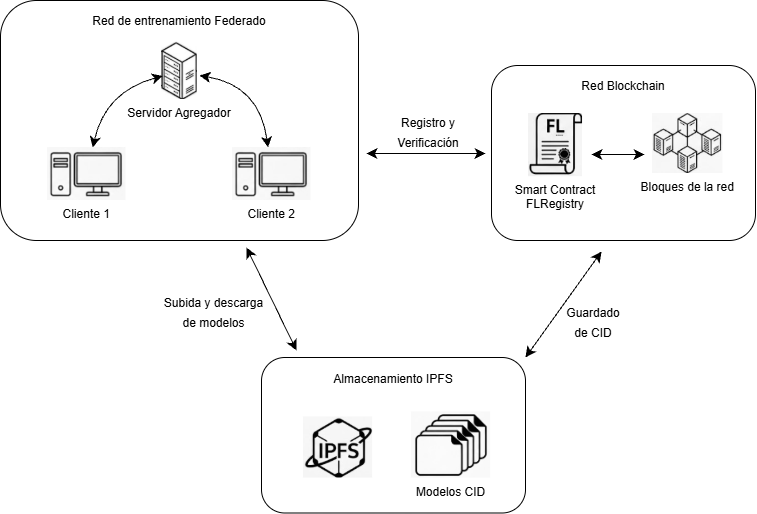
\includegraphics[width=0.88\textwidth]{figuras/ArqSistema.png}
    \caption{Arquitectura general del sistema híbrido: desacoplamiento entre el cómputo federado (Flower), el almacenamiento de pesos fuera de cadena (IPFS) y el registro inmutable de trazabilidad (Hyperledger Besu con IBFT 2.0).}
    \label{fig:arq_sistema}
\end{figure*}

\subsection{Diseño del Smart Contract: FLRegistry}
El componente de gobernanza y auditoría lógica se implementa mediante el contrato inteligente \texttt{FLRegistry}, codificado en Solidity (versión \texttt{0.8.10}). Su misión es registrar un historial criptográfico determinista de cada ronda sin albergar matrices numéricas masivas on-chain.
\\

\subsubsection{Estructuras de datos y persistencia}
La entidad nuclear del contrato es la estructura \texttt{ModelRound}, definida como:
\begin{verbatim}
struct ModelRound {
    uint256 roundNum;
    string modelHash;
    address author;
    uint256 timestamp;
}
\end{verbatim}
donde \texttt{roundNum} indexa la iteración federada, \texttt{modelHash} almacena el CID o digest SHA-256 del artefacto del modelo, \texttt{author} guarda la dirección pública Ethereum del emisor (\texttt{msg.sender}) y \texttt{timestamp} captura la marca temporal del bloque validado.
\\

El estado del contrato se organiza mediante dos tablas hash (\textit{mappings}) complementarias:
\begin{itemize}
    \item \texttt{mapping(uint256 => ModelRound) public \\ history}: almacena de forma secuencial los modelos globales agregados por el servidor al término de cada ronda $t$.
    \item \texttt{mapping(uint256 => mapping(address => \\ ModelRound)) public clientHistory}: indexa las contribuciones locales individuales de cada cliente en cada ronda, posibilitando la auditoría forense granular de las participaciones.
\end{itemize}

Adicionalmente, se mantienen los punteros de estado \texttt{latestRound} y el indicador booleano \texttt{hasModel} para optimizar lecturas directas de acceso constante sin requerir iteraciones sobre el almacenamiento persistente.
\\

\subsubsection{Primitivas de escritura y control de acceso}
El contrato expone dos métodos transaccionales que alteran el estado y emiten el evento desacoplado \texttt{ModelUpdated}:
\begin{itemize}
    \item \texttt{registerClientModel(uint256 round, string memory hash)}: Invocado por cada cliente $k$ tras concluir su entrenamiento local, registrando de forma inmutable el CID de su contribución junto a su dirección Ethereum (\texttt{msg.sender}).
    \item \texttt{updateModel(uint256 round, string memory hash)}: Invocado operacionalmente por el servidor agregador tras converger el algoritmo de agregación. Para salvaguardar la gobernanza de la red y evitar que cualquier participante no autorizado o nodo malicioso pueda registrar modelos globales maliciosos, la función se protege mediante el modificador de control de acceso \texttt{onlyServer}:
    \begin{verbatim}
modifier onlyServer() {
    require(msg.sender == serverAddress, 
            "Emisor no autorizado");
    _;
}
    \end{verbatim}
    donde \texttt{serverAddress} se inicializa en el constructor del contrato con la clave pública del servidor agregador autorizado (pudiendo ser delegada o actualizada mediante esquemas de gobernanza multifirma del consorcio). De este modo, la EVM revierte de manera determinista cualquier invocación no autorizada de \texttt{updateModel}.
\end{itemize}

\subsubsection{Primitivas de lectura y verificación}
Para no sobrecargar la red con costes de ejecución, las consultas de verificación se implementan como funciones \texttt{view}, las cuales se resuelven localmente en el nodo RPC sin consumir gas:
\begin{itemize}
    \item \texttt{getLastModel()}: Permite a cualquier cliente recuperar el CID del último modelo global consolidado y su marca de tiempo.
    \item \texttt{getClientModel(uint256 round, address client)}: Permite al servidor y a auditores externos cotejar el CID reportado por un cliente frente a su registro on-chain firmado.
\end{itemize}

\subsubsection{Generalización y desacoplamiento del modelo}
Conviene destacar que el diseño del marco es conceptual y operativamente agnóstico a la topología de la red neuronal, a la modalidad de los datos y al framework de aprendizaje empleado. Debido a que el contrato \texttt{FLRegistry} gestiona exclusivamente cadenas de longitud uniforme (los CIDs de IPFS y los resúmenes SHA-256), el coste de gas en la EVM permanece predecible y desacoplado de la complejidad del modelo, independientemente de si los parámetros corresponden a un clasificador ligero, una red convolucional profunda o una arquitectura basada en Transformers. Asimismo, el plano de almacenamiento IPFS maneja los pesos serializados como secuencias de bytes genéricas, posibilitando que el protocolo de doble verificación sea extrapolable a diversas modalidades (datos tabulares, series temporales, señales acústicas o visión artificial) y algoritmos de optimización federada.

\subsection{Flujo Operacional y Doble Verificación Cruzada}
El ciclo de vida del entrenamiento federado se estructura en una fase de inicialización única seguida de un protocolo iterativo con verificación bidireccional estricta, como se resume a continuación:
\\

\subsubsection{Fase 0: Arranque y Modelo Base (Ronda 0)}
Antes de iniciar la concurrencia:
\begin{enumerate}
    \item Se inicializa la red Besu con consenso IBFT 2.0 y el daemon IPFS.
    \item Se despliega \texttt{FLRegistry} registrando su dirección y ABI en un descriptor JSON distribuido.
    \item El servidor instancia los pesos iniciales $w^{(0)}$, los serializa y los almacena en IPFS, recibiendo un CID inicial $\text{CID}_0$.
    \item El servidor ejecuta \texttt{updateModel(0, }$\text{CID}_0$\texttt{)}, fijando el punto de partida auditable para todos los participantes. \\
\end{enumerate}

\subsubsection{Fase 1: Verificación Descendente (Cliente protege frente a Servidor)}
Al recibir la señal de inicio de ronda junto con los pesos candidatos $w_{cand}^{(t)}$ vía gRPC (Figura~\ref{fig:flujo_cliente_verif}):
\begin{enumerate}
    \item El cliente consulta la Blockchain invocando \texttt{getLastModel()} y obtiene el $\text{CID}_{reg}^{(t-1)}$ oficial.
    \item El cliente descarga el modelo referenciado desde IPFS y realiza una verificación bit a bit tensor por tensor frente a $w_{cand}^{(t)}$.
    \item Si se detecta cualquier discrepancia entre los pesos entregados y el compromiso sellado en la cadena, el cliente \textbf{aborta el entrenamiento inmediatamente}, neutralizando ataques donde un servidor comprometido intente inyectar modelos sesgados selectivamente a clientes concretos.
\end{enumerate}

\begin{figure}[H]
    \centering
    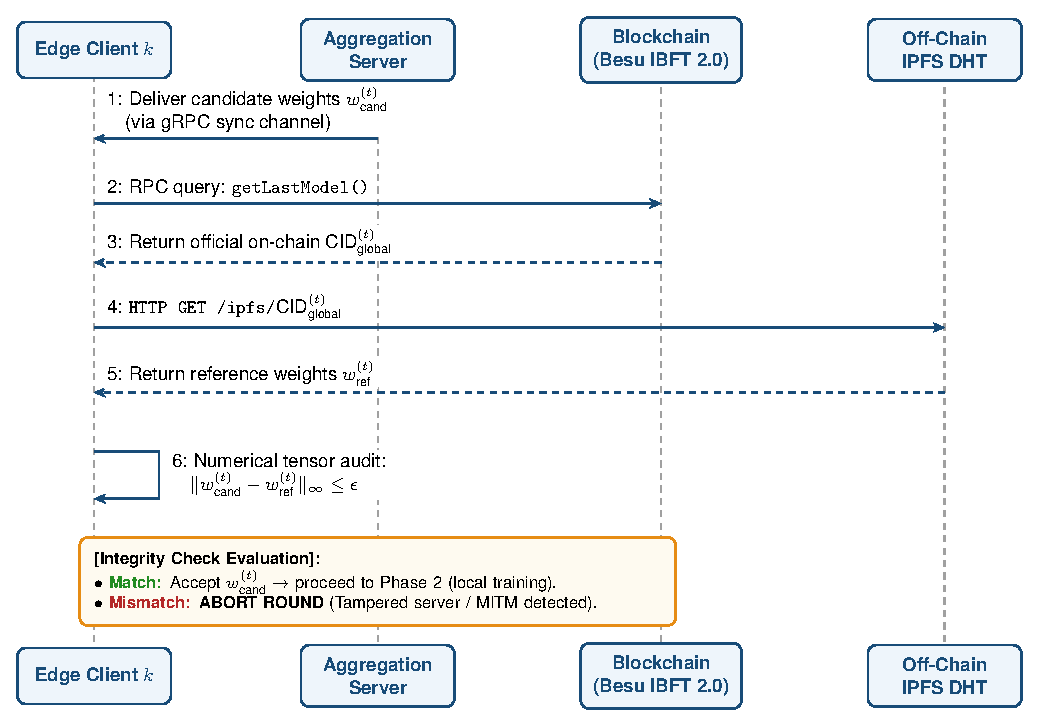
\includegraphics[width=\columnwidth]{figuras/flujo_fase1_verificacion_descendente.pdf}
    \caption{Fase 1: Verificación descendente en el cliente: cotejo del modelo recibido frente al CID registrado on-chain y descargado de IPFS.}
    \label{fig:flujo_cliente_verif}
\end{figure}

\subsubsection{Fase 2: Entrenamiento Local y Registro de Contribución}
Si la comprobación previa es satisfactoria (Figura~\ref{fig:flujo_cliente_entreno}):
\begin{enumerate}
    \item El cliente ejecuta el entrenamiento local con su partición privada de datos.
    \item Serializa los nuevos pesos locales $w_k^{(t)}$ y los almacena en IPFS, obteniendo $\text{CID}_k^{(t)}$.
    \item Emite una transacción firmada con su clave privada invocando \texttt{registerClientModel(}$t$, $\text{CID}_k^{(t)}$\texttt{)} y aguarda el recibo (\textit{receipt}) de inclusión en el bloque IBFT 2.0.
    \item Retorna a Flower los parámetros junto con el identificador $\text{CID}_k^{(t)}$ y su clave pública.
\end{enumerate}

\begin{figure}[H]
    \centering
    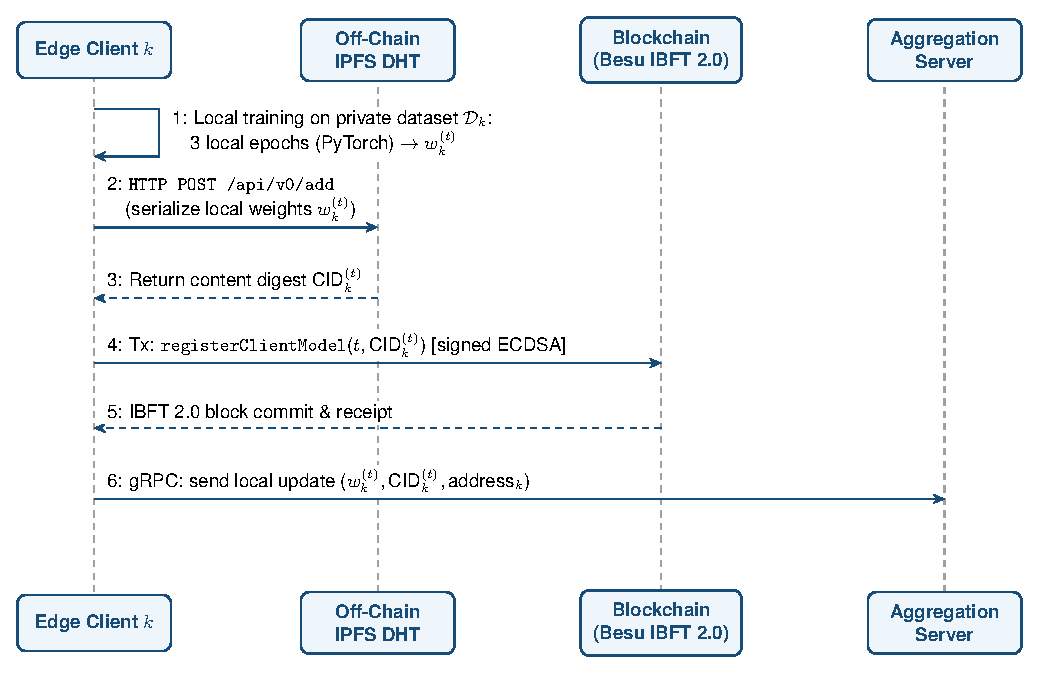
\includegraphics[width=\columnwidth]{figuras/flujo_fase2_entrenamiento_registro.pdf}
    \caption{Fase 2: Entrenamiento local en el cliente, subida de pesos a IPFS y transacción firmada a Hyperledger Besu.}
    \label{fig:flujo_cliente_entreno}
\end{figure}

\subsubsection{Fase 3: Verificación Ascendente y Agregación Global}
Al recibir las actualizaciones de los clientes en el servidor agregador (Figura~\ref{fig:flujo_servidor_agregacion}):
\begin{enumerate}
    \item Para cada cliente $k$, el servidor recibe la carga útil de los parámetros $w_k^{(t)}$ junto con el identificador $\text{CID}_{k,\text{gRPC}}^{(t)}$ y la dirección pública del cliente $\text{address}_k$.
    \item \textbf{Cálculo de integridad local:} El servidor computa de forma determinista el resumen criptográfico del vector de pesos recibido en memoria: $\text{CID}_{k,\text{calc}}^{(t)} = \text{Hash}(w_k^{(t)})$.
    \item \textbf{Consulta on-chain y doble verificación cruzada:} El servidor consulta la función de sólo lectura \texttt{getClientModel($t$, address$_k$)} en \texttt{FLRegistry}, recuperando $\text{CID}_{k,\text{onchain}}^{(t)}$, y valida la condición estricta de doble coincidencia:
    \begin{equation}
    \text{CID}_{k,\text{calc}}^{(t)} == \text{CID}_{k,\text{gRPC}}^{(t)} == \text{CID}_{k,\text{onchain}}^{(t)}
    \end{equation}
    Esta doble comprobación neutraliza dos vectores de ataque complementarios: si un cliente malicioso registrara un CID válido en Besu pero enviara pesos adulterados por gRPC, o si un atacante en red modificara los parámetros en tránsito, $\text{CID}_{k,\text{calc}}^{(t)} \neq \text{CID}_{k,\text{onchain}}^{(t)}$; análogamente, si el CID transmitido por gRPC no se correspondiera con la transacción firmada en Besu, la comprobación fallaría de inmediato. En cualquier caso de discrepancia, la contribución es descartada de forma preventiva antes de la agregación.
    \item Aplica la agregación ponderada FedAvg únicamente sobre las contribuciones debidamente validadas:
    \begin{equation}
    w^{(t+1)} = \sum_{k \in \mathcal{K}_{valid}} \frac{n_k}{n_{valid}} \, w_k^{(t)}
    \end{equation}
    donde $n_k$ representa el número de muestras locales aportadas por el cliente $k$ y $n_{valid} = \sum_{k \in \mathcal{K}_{valid}} n_k$.
    \item Sube el nuevo modelo consolidado a IPFS, obteniendo $\text{CID}_{global}^{(t+1)}$, y lo sella en Besu invocando \texttt{updateModel(}$t+1$, $\text{CID}_{global}^{(t+1)}$\texttt{)}. Dado que \texttt{updateModel} está restringida por el modificador \texttt{onlyServer}, ningún tercero ajeno al agregador designado puede sobrescribir el modelo global.
\end{enumerate}

\begin{figure}[H]
    \centering
    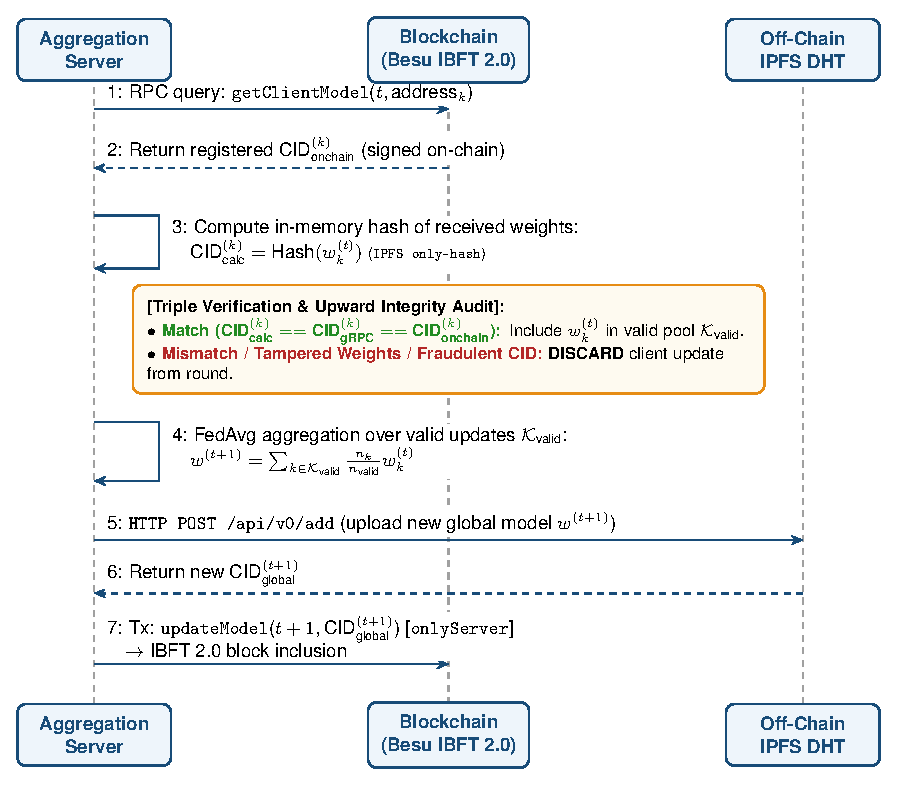
\includegraphics[width=\columnwidth]{figuras/flujo_fase3_verificacion_agregacion.pdf}
    \caption{Fase 3: Verificación ascendente en el servidor: validación de integridad tensorial, verificación on-chain, agregación FedAvg y sellado global de ronda.}
    \label{fig:flujo_servidor_agregacion}
\end{figure}

\subsection{Auditoría Ex-Post y Verificabilidad de FedAvg}
\label{subsec:auditoria_fedavg}
Una propiedad arquitectónica diferencial que se deriva del desacoplamiento híbrido propuesto es la capacidad de verificar de forma determinista y retrospectiva (\textit{ex-post}) el comportamiento del servidor agregador. En los marcos federados convencionales, el servidor actúa como una caja negra de confianza: los clientes deben asumir que los pesos agregados $w^{(t+1)}$ se computaron aplicando honestamente la media ponderada sobre las contribuciones recibidas, sin introducir sesgos no autorizados, omitir clientes arbitrariamente o insertar puertas traseras encubiertas.

En nuestra arquitectura, para cada ronda $t$, quedan registrados de forma inmutable en la cadena de bloques:
\begin{enumerate}
    \item El conjunto de participantes validados $\mathcal{K}_t$ y sus direcciones de cuenta Ethereum.
    \item Los CIDs $\text{CID}_k^{(t)}$ firmados individualmente por cada cliente en \texttt{clientHistory}.
    \item Los volúmenes de datos muestrales $n_k$ correspondientes a cada cliente.
    \item El CID del modelo global resultante $\text{CID}_{global}^{(t+1)}$ registrado por el servidor en \texttt{history}.
\end{enumerate}

Gracias a este registro exhaustivo, cualquier nodo cliente de la federación o una entidad auditora externa independiente puede ejecutar en cualquier instante una verificación determinista de la agregación sin requerir acceso a los conjuntos de datos privados:
\begin{enumerate}
    \item \textbf{Recuperación de artefactos:} El auditor consulta en Besu las direcciones participantes y sus CIDs correspondientes a la ronda $t$, y descarga desde IPFS los vectores de pesos $w_k^{(t)}$.
    \item \textbf{Cotejo de integridad de entrada:} Verifica que para cada cliente $k \in \mathcal{K}_t$, el hash de los pesos descargados coincide con $\text{CID}_k^{(t)}$ sellado en el contrato.
    \item \textbf{Reconstrucción de la agregación:} Aplica formalmente la fórmula determinista de FedAvg:
    \begin{equation}
    \hat{w}^{(t+1)} = \sum_{k \in \mathcal{K}_t} \frac{n_k}{\sum_{j \in \mathcal{K}_t} n_j} \, w_k^{(t)}
    \end{equation}
    \item \textbf{Cotejo del modelo global:} Serializa $\hat{w}^{(t+1)}$ y genera su identificador de contenido $\text{CID}_{audit}^{(t+1)} = \text{Hash}(\hat{w}^{(t+1)})$. A continuación, compara $\text{CID}_{audit}^{(t+1)}$ frente al $\text{CID}_{global}^{(t+1)}$ registrado en \texttt{FLRegistry}.
\end{enumerate}
Si $\text{CID}_{audit}^{(t+1)} \neq \text{CID}_{global}^{(t+1)}$, queda demostrada criptográficamente de manera pública, no repudiable y reproducible la deshonestidad del servidor (ya sea por manipulación de pesos, alteración arbitraria de las ponderaciones $n_k$, o inyección de parámetros maliciosos). Esta verificabilidad transforma la figura del agregador centralizado en un orquestador estrictamente auditable y sujeto a responsabilidad demostrable (\textit{accountability}).

\subsection{Modelo de Amenazas y Alcance de Seguridad}
\label{subsec:modelo_amenazas}
Para delimitar con precisión las garantías provistas por el marco propuesto, se define a continuación el modelo de amenazas considerado, distinguiendo explícitamente entre las vulnerabilidades mitigadas por el diseño arquitectónico y aquellas que quedan formalmente fuera del alcance.

\subsubsection{Amenazas Mitigadas (In-Scope)}
\begin{itemize}
    \item \textbf{Manipulación en tránsito (\textit{Man-in-the-Middle})}: Un adversario en red que intercepte el canal gRPC e intente modificar los tensores locales enviados al servidor o los pesos globales distribuidos a los clientes. Dicha alteración es detectada de forma inmediata gracias al cotejo tensorial bit a bit y a la verificación frente al CID sellado on-chain.
    \item \textbf{Bifurcación y equivocación del servidor (\textit{Server Equivocation / Split-View})}: Un servidor malicioso que intente engañar a clientes específicos enviándoles modelos globales diferentes o adulterados. Dado que los clientes únicamente aceptan pesos cuyo CID coincide unívocamente con el último estado publicado en \texttt{FLRegistry}, cualquier intento de distribución divergente es detectado y bloqueado localmente.
    \item \textbf{Inyección de modelos globales por terceros no autorizados}: Intentos por parte de nodos disidentes o atacantes externos de registrar modelos globales falsos en la Blockchain quedan neutralizados en la EVM mediante el modificador de control de acceso \texttt{onlyServer}.
    \item \textbf{Repudio de contribuciones}: La firma digital basada en criptografía de curva elíptica (ECDSA secp256k1) vinculada a cada transacción en Hyperledger Besu impide que un cliente niegue haber generado o subido una actualización registrada a su nombre.
\end{itemize}

\subsubsection{Amenazas Fuera de Alcance (Out-of-Scope) y Límites del Sistema}
\begin{itemize}
    \item \textbf{Envenenamiento semántico legítimamente firmado (\textit{Semantic Data/Model Poisoning})}: Si un participante genera un modelo malicioso (por ejemplo, mediante técnicas de volteo de etiquetas, \textit{label flipping}, o puertas traseras) a partir de sus propios datos y firma correctamente la transacción en Besu cumpliendo el protocolo, el sistema garantiza la trazabilidad y la atribución no repudiable de la autoría, pero la verificación criptográfica no evalúa la calidad estadística de los gradientes. La defensa ante esta amenaza debe complementarse mediante algoritmos de agregación estadística bizantina robusta (e.g., Krum~\cite{blanchard2017byzantine}, Median o Trimmed Mean) o auditorías forenses posteriores sobre las contribuciones registradas.
    \item \textbf{Compromiso y sustracción de claves privadas (\textit{Key Compromise})}: La validez de las garantías criptográficas descansa sobre la premisa de que las claves privadas de los participantes están debidamente custodiadas. En entornos de producción industrial, este vector exige el empleo de módulos de seguridad de hardware (HSM) o enclaves de ejecución segura (TEE).
    \item \textbf{Ataques de inferencia y reconstrucción de datos crudos (\textit{Inference / Gradient Inversion})}: El protocolo garantiza integridad y procedencia, pero no implementa por defecto mecanismos de Privacidad Diferencial (DP) ni Cómputo Seguro Multipartito (SMPC) sobre los gradientes compartidos.
\end{itemize}

\subsubsection{Privacidad y Exposición de Pesos en IPFS}
En una instancia estándar y pública de IPFS, cualquier participante que conozca el identificador de contenido (CID) podría recuperar los tensores del modelo y potencialmente aplicar técnicas de inferencia para extraer información sobre los datos de entrenamiento locales. Para mitigar esta exposición en entornos consorciados con altos requisitos de confidencialidad (e.g., flotas vehiculares o historiales clínicos), el marco admite dos soluciones de endurecimiento complementarias:
\begin{enumerate}
    \item \textbf{Despliegue de red privada IPFS (\textit{Private Swarm})}: Configuración del daemon IPFS en modo de enjambre privado mediante la definición de una clave compartida (\texttt{swarm.key}) y la variable de entorno \texttt{LIBP2P\_FORCE\_PNET=1}. Esta directiva impide que cualquier nodo ajeno al consorcio se conecte a la red peer-to-peer o resuelva bloques de almacenamiento fuera de los nodos autorizados.
    \item \textbf{Cifrado simétrico en reposo (\textit{Payload Encryption})}: Cifrado de los vectores de parámetros serializados (mediante AES-256-GCM) de forma previa a su subida a IPFS. La clave simétrica de descifrado puede gestionarse mediante esquemas de cifrado híbrido asimétrico dirigidos exclusivamente a las claves públicas de los miembros autorizados del consorcio o esquemas de Cifrado Basado en Atributos (ABE).
\end{enumerate}

% !TeX root = ../main.tex
\section{Implementación y Entorno Experimental}
\label{sec:implementacion}

Con el fin de aislar y evaluar cuantitativamente el sobrecoste introducido por la capa de trazabilidad y auditoría, se desplegó un banco de pruebas experimental representativo de un entorno de computación distribuida vehicular.

\subsection{Infraestructura de Hardware y Software}
La evaluación empírica se llevó a cabo utilizando dos estaciones físicas interconectadas en la misma red de área local (LAN), cuyas especificaciones técnicas se detallan en la Tabla~\ref{tab:testbed_hardware}:
\begin{itemize}
    \item \textbf{Estación 1 (Nodo Central)}: Aloja el servidor agregador Flower, el nodo RPC principal de la red Besu y el nodo de almacenamiento IPFS.
    \item \textbf{Estación 2 (Nodos de Borde / Clientes)}: Aloja y ejecuta los clientes de entrenamiento federado (\textit{members} 2 y 3).
\end{itemize}

\begin{table}[H]
\centering
\caption{Especificaciones del banco de pruebas experimental.}
\label{tab:testbed_hardware}
\resizebox{\columnwidth}{!}{%
\begin{tabular}{lll}
\toprule
\textbf{Parámetro} & \textbf{Estación 1 (Servidor/RPC)} & \textbf{Estación 2 (Clientes)} \\
\midrule
Procesador & Intel Core i5-1135G7 & Intel Core i7-9700 \\
Frecuencia base & 2,40 GHz & 3,00 GHz \\
Núcleos / Hilos & 4 núcleos / 8 hilos & 8 núcleos / 8 hilos \\
Memoria RAM & 7,6 GB (asignada en WSL2) & 8,0 GB \\
Sistema Operativo & Ubuntu 22.04 LTS (WSL2) & Windows 11 \\
\bottomrule
\end{tabular}%
}
\end{table}

El stack de software está compuesto por Hyperledger Besu con soporte de transacciones privadas mediante Tessera, orquestado mediante Docker Compose; el daemon IPFS Kubo (\texttt{v0.32.1}); Python \texttt{3.12} con PyTorch~\cite{paszke2019pytorch} para la inferencia y optimización neuronal; Flower (\texttt{flwr})~\cite{beutel2020flower} para la coordinación gRPC de la federación; y la biblioteca \texttt{web3.py} para la conectividad JSON-RPC con la EVM. Todos los contratos inteligentes, configuraciones de red y scripts de orquestación se encuentran disponibles en el repositorio público~\url{https://github.com/dpz6-ua/Blockchain_ML}.

Las dos estaciones se encuentran comunicadas a través de un enlace de red de área local inalámbrico (Wi-Fi 802.11ac a 5~GHz), registrando una latencia media de ida y vuelta (\textit{RTT ping}) de $3{,}8 \pm 1{,}1$~ms y un ancho de banda sostenido de 100~Mbps. El tamaño del modelo neuronal serializado (\texttt{NetCliente}) es de exactamente $1{,}95$~MB en formato binario. Para garantizar un rendimiento óptimo en la capa de almacenamiento distribuido, la subida a IPFS se efectúa mediante la API HTTP en el endpoint \texttt{/api/v0/add?pin=false}, lo que permite registrar y generar el identificador CID en memoria local en milisegundos.

\subsection{Modelo Neuronal y Conjunto de Datos Vehicular}
Como caso de uso para simular un sistema de asistencia a la conducción en vehículos conectados y autónomos (CAV), se adoptó el dataset de clasificación de eventos de tráfico del grupo CloudLab-AIA~\cite{cloudlabaia_flblockchain}. 

El problema consiste en una tarea de clasificación multiclase orientada a la detección en carretera con cuatro categorías:
\begin{enumerate}
    \item Accidente vial (\texttt{accident}).
    \item Congestión o tráfico denso (\texttt{dense\_traffic}).
    \item Condiciones meteorológicas adversas (\texttt{meteorology}).
    \item Flujo de tráfico fluido (\texttt{sparse\_traffic}).
\end{enumerate}

El conjunto de datos comprende un total de 3.415 imágenes distribuidas en: meteorología adversa (1.027), tráfico fluido (947), tráfico denso (778) y accidentes (663). Las imágenes se preprocesan mediante reescalado a una resolución de $32 \times 32$ píxeles en tres canales cromáticos (RGB) y normalización estándar. Para preservar la comparabilidad estadística y eliminar sesgos de distribución, el conjunto de datos se reparte entre los $K=2$ clientes según un esquema independiente e idénticamente distribuido (IID).

El modelo implementado (\texttt{NetCliente}) es una red neuronal convolucional (CNN) estructurada en dos bloques convolucionales consecutivos (con kernels de $3 \times 3$, función de activación ReLU y submuestreo por \textit{Max Pooling}), seguidos de dos capas densas completamente conectadas (\textit{fully connected}) que proyectan el vector de características hacia las 4 neuronas de salida. El entrenamiento se realiza mediante la función de pérdida de entropía cruzada (\textit{Cross-Entropy Loss}) y el algoritmo de optimización Adam con una tasa de aprendizaje $\eta = 10^{-3}$, configurando un tamaño de lote (\textit{batch size}) de 16 muestras en entrenamiento y 32 en evaluación, 3 épocas locales de entrenamiento por ronda y un horizonte total de 30 rondas federadas.

Es importante remarcar que el propósito primordial de este estudio no radica en diseñar el modelo más óptimo ni en maximizar su precisión de clasificación, sino en utilizar la arquitectura de aprendizaje federado como un banco de pruebas realista para generar y analizar métricas cuantitativas del sistema (sobrecoste temporal, escalabilidad y consumo de gas). La optimización del modelo (ajuste de hiperparámetros, mitigación del sobreajuste o empleo de arquitecturas más profundas) se plantea deliberadamente como trabajo futuro, actuando aquí la red neuronal como una carga de trabajo experimental de referencia.

\subsection{Matriz de Configuraciones Experimentales}
Para desglosar y desacoplar de forma analítica el impacto individual de cada componente, se diseñaron cinco configuraciones experimentales (E1 a E5), resumidas en la Tabla~\ref{tab:configuraciones}.

\begin{table}[H]
\centering
\caption{Matriz de configuraciones experimentales evaluadas.}
\label{tab:configuraciones}
\resizebox{\columnwidth}{!}{%
\begin{tabular}{ccccc}
\toprule
\textbf{ID Exp.} & \textbf{Estaciones} & \textbf{Capa Blockchain} & \textbf{Validadores} & \textbf{Objetivo} \\
\midrule
E1 & 1 & Sí & 4 & Sobrecarga BC local \\
E2 & 1 & No & --- & Baseline local \\
E3 & 2 & No & --- & Baseline distribuido \\
E4 & 2 & Sí & 4 & Sobrecarga BC distribuida \\
E5 & 2 & Sí & 7 & Escalabilidad IBFT 2.0 \\
\bottomrule
\end{tabular}%
}
\end{table}

Este diseño metodológico permite efectuar comparaciones controladas de una sola variable:
\begin{itemize}
    \item \textbf{Coste directo de Blockchain}: Comparación de E1 vs. E2 en entorno monomáquina, y de E4 vs. E3 en entorno distribuido en red.
    \item \textbf{Efecto de la distribución física}: Comparación de E2 vs. E3 (sin Blockchain) y de E1 vs. E4 (con Blockchain de 4 validadores).
    \item \textbf{Escalado del consenso BFT}: Comparación de E4 (4 validadores) vs. E5 (7 validadores), evaluando la penalización de latencia al elevar la tolerancia a fallos de $f=1$ a $f=2$.
\end{itemize}


% !TeX root = ../main.tex
\section{Evaluación Experimental y Resultados}
\label{sec:evaluacion}

En esta sección se analiza cuantitativamente el comportamiento del sistema a lo largo del banco de pruebas experimental, respondiendo a las preguntas de investigación formuladas: el sobrecoste temporal de la capa de auditoría, el desacoplamiento de recursos físicos, la escalabilidad del consenso bizantino IBFT~2.0, la resiliencia empírica frente a ataques de adulteración y la previsibilidad del consumo de gas en la EVM. Con el objetivo de afianzar la solidez, robustez y reproducibilidad experimental, cada una de las cinco configuraciones experimentales ($E_1$ a $E_5$) fue evaluada a lo largo de 3 ejecuciones independientes completas de 30 rondas cada una, totalizando un corpus de 15 ejecuciones y 450 rondas federadas ($N_{\text{total}} = 450$).

\subsection{Convergencia del Modelo y Análisis de Pérdida}
La Figura~\ref{fig:convergencia} ilustra la evolución de la función de pérdida de entropía cruzada en el conjunto de validación durante las 30 iteraciones federadas.

\begin{figure}[H]
    \centering
    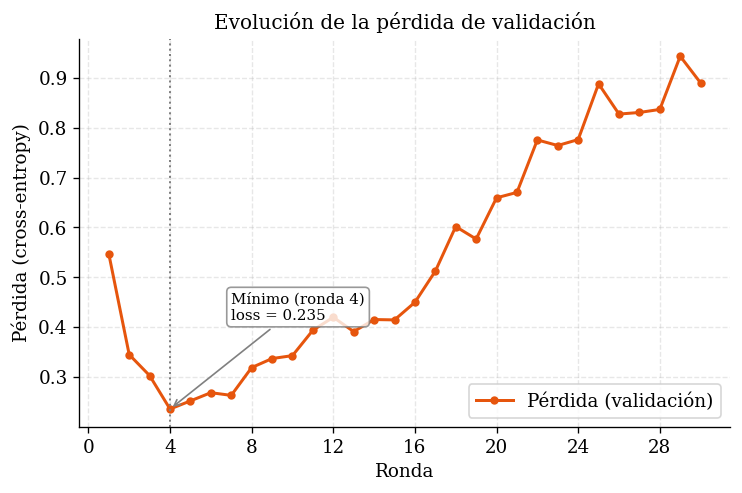
\includegraphics[width=\columnwidth]{figuras/convergencia_loss.png}
    \caption{Evolución de la pérdida de validación (\textit{cross-entropy}) a lo largo de las 30 rondas federadas.}
    \label{fig:convergencia}
\end{figure}

El modelo muestra un rápido aprendizaje inicial, alcanzando su mínimo de pérdida en la ronda 4 ($\mathcal{L} \approx 0{,}24$) con una precisión de clasificación que se estabiliza en el $97\%$. A partir de dicho punto, la pérdida experimenta un incremento gradual y sostenido hasta situarse en torno a $0{,}90$ hacia el final del ciclo. Este comportamiento representa un caso paradigmático de sobreajuste (\textit{overfitting}) provocado por el régimen de 90 épocas acumuladas (3 épocas locales $\times$ 30 rondas federadas) sobre un conjunto de entrenamiento acotado, donde la red incrementa excesivamente su confianza en predicciones.

El mínimo de pérdida en la ronda 4 sugiere que la incorporación de técnicas como la parada temprana (\textit{early stopping}) habría detenido el entrenamiento en ese instante, logrando una versión más ajustada del clasificador. Sin embargo, se mantuvieron de forma deliberada las 30 rondas predefinidas porque el objetivo central de esta investigación no es optimizar el modelo de IA ni perseguir su punto de máxima eficiencia, sino someter la infraestructura de aprendizaje federado a una carga constante para extraer métricas cuantitativas reproducibles (latencia por ronda, tiempo de confirmación y coste de gas). De este modo, la optimización fina del modelo se pospone como trabajo futuro.

Es fundamental enfatizar que \textbf{la curva de convergencia es estrictamente idéntica con o sin la presencia de Blockchain}. Dado que la capa de trazabilidad opera exclusivamente en la verificación e indexación criptográfica fuera de cadena y no interfiere en los tensores ni en los gradientes de FedAvg, la dinámica de entrenamiento se mantiene inalterada.

\subsection{Formalización Matemática de Métricas de Rendimiento}
Con el fin de aislar de forma unívoca la latencia impuesta por cada componente del sistema, el tiempo total por ronda en los nodos de borde ($T_{\text{client}}$) y en el servidor agregador ($T_{\text{server}}$) en la iteración $t$ se define analíticamente como:
\begin{align}
T_{\text{client}}^{(t)} &= t_{\text{verif\_desc}}^{(t)} + t_{\text{train}}^{(t)} + t_{\text{ipfs\_up}}^{(t)} + t_{\text{tx\_besu}}^{(t)} \label{eq:t_client} \\
T_{\text{server}}^{(t)} &= t_{\text{wait}}^{(t)} + t_{\text{verif\_asc}}^{(t)} + t_{\text{fedavg}}^{(t)} \nonumber \\
&\quad + t_{\text{ipfs\_global}}^{(t)} + t_{\text{block\_confirm}}^{(t)} \label{eq:t_server}
\end{align}
donde $t_{\text{verif\_desc}}$ representa la comprobación local contra el CID de Besu; $t_{\text{train}}$, el tiempo de cálculo de gradientes con PyTorch; $t_{\text{ipfs\_up}}$, la publicación binaria de pesos; $t_{\text{tx\_besu}}$, la emisión y confirmación de \texttt{registerClientModel}; $t_{\text{wait}}$, la ventana de recepción gRPC; $t_{\text{verif\_asc}}$, la validación en \texttt{getClientModel}; $t_{\text{fedavg}}$, la agregación matricial; y $t_{\text{block\_confirm}}$, la confirmación del bloque IBFT~2.0 tras invocar \texttt{updateModel}.

Es crucial destacar la complementariedad entre ambas perspectivas temporales:
\begin{itemize}
    \item \textbf{Tiempo de ciclo en el cliente ($T_{\text{client}}$, reportado en la Tabla~\ref{tab:tiempos_resumen}):} Cuantifica la duración de la computación y comunicación local en los nodos de borde (vehículos), desde que reciben el modelo global hasta que sellan su contribución en la Blockchain. Esta métrica gobierna la autonomía operativa de los clientes y mantiene la comparabilidad directa con los estudios previos~\cite{cloudlabaia_flblockchain}.
    \item \textbf{Tiempo de ronda extremo a extremo en el servidor ($T_{\text{server}}$, desglosado en la Tabla~\ref{tab:desglose_fases}):} Engloba la totalidad del ciclo orquestado por el agregador central, incorporando la sincronización gRPC de todos los clientes concurrentes y la inclusión en bloque del nuevo modelo global mediante \texttt{updateModel} ($\approx 2{,}8\text{--}5{,}1$~s adicionales por ronda).
\end{itemize}

Para medir el sobrecoste relativo ($\Delta_{\text{overhead}}$) entre una configuración con seguridad $E_{\text{BC}}$ y su respectiva línea base $E_{\text{base}}$, se emplea la mediana de las distribuciones:
\begin{equation}
\Delta_{\text{overhead}} = \frac{\text{Med}(T_{E_{\text{BC}}}) - \text{Med}(T_{E_{\text{base}}})}{\text{Med}(T_{E_{\text{base}}})} \times 100 \quad [\%] \label{eq:overhead}
\end{equation}

En cuanto al rigor metodológico del análisis estadístico, el diseño experimental considera como unidades muestrales independientes las \textbf{15 ejecuciones completas} ($N_{\text{runs}} = 3$ repeticiones independientes por cada una de las 5 configuraciones). Las 30 rondas federadas consecutivas de cada ejecución no se presentan como observaciones independientes idénticamente distribuidas (i.i.d.), ya que cada iteración $t+1$ depende intrínsecamente del estado paramétrico y las condiciones del sistema en la ronda $t$. Por consiguiente, las 450 rondas totales ($90$ por configuración) se emplean para el análisis descriptivo longitudinal y la visualización de trayectorias (Figura~\ref{fig:tiempo_todas}), mientras que la reproducibilidad inter-ejecución se cuantifica a través del Error Estándar ($SE$) entre las medias de las ejecuciones independientes ($SE = \sigma_{\text{runs}} / \sqrt{N_{\text{runs}}}$).

\subsection{Visión General del Rendimiento Temporal Consolidado}
La Tabla~\ref{tab:tiempos_resumen} sintetiza el tiempo de ciclo por ronda en los nodos de borde ($T_{\text{client}}$) a lo largo de las 15 ejecuciones independientes (3 por configuración, totalizando 90 rondas por entorno para análisis descriptivo continuo), reportando la mediana, media, desviación típica inter-ejecución ($\sigma_{\text{runs}}$) y error estándar ($SE = \sigma_{\text{runs}} / \sqrt{3}$). Asimismo, la Figura~\ref{fig:tiempo_todas} refleja la serie temporal continua a lo largo de las rondas.

\begin{table}[H]
\centering
\caption{Tiempo de ciclo por ronda en los nodos de borde ($T_{\text{client}}$) consolidado ($15$ ejecuciones independientes, $3$ por configuración, $30$ rondas/run). Los valores de $\sigma_{\text{runs}}$ y $SE$ cuantifican la dispersión y el error estándar entre las medias de las $3$ ejecuciones independientes ($SE = \sigma_{\text{runs}} / \sqrt{3}$).}
\label{tab:tiempos_resumen}
\resizebox{\columnwidth}{!}{%
\begin{tabular}{@{}cccccccc@{}}
\toprule
\textbf{Exp.} & \textbf{Máq.} & \textbf{Configuración} & \textbf{Runs} & \textbf{Mediana (s)} & \textbf{Media (s)} & \textbf{$\sigma_{\text{runs}}$ (s)} & \textbf{SE (s)} \\
\midrule
$E_1$ & 1 & 4 val · con BC & 3 & \textbf{85,42} & 97,09 & 20,01 & 11,55 \\
$E_2$ & 1 & Baseline sin BC & 3 & \textbf{75,70} & 76,45 & 1,65 & 0,95 \\
\midrule
$E_3$ & 2 & Baseline sin BC & 3 & \textbf{66,62} & 67,62 & 2,29 & 1,32 \\
$E_4$ & 2 & 4 val · con BC & 3 & \textbf{72,96} & 73,29 & 1,28 & 0,74 \\
$E_5$ & 2 & 7 val · con BC & 3 & \textbf{73,35} & 74,40 & 0,54 & 0,31 \\
\bottomrule
\end{tabular}%
}
\end{table}

\begin{figure}[H]
    \centering
    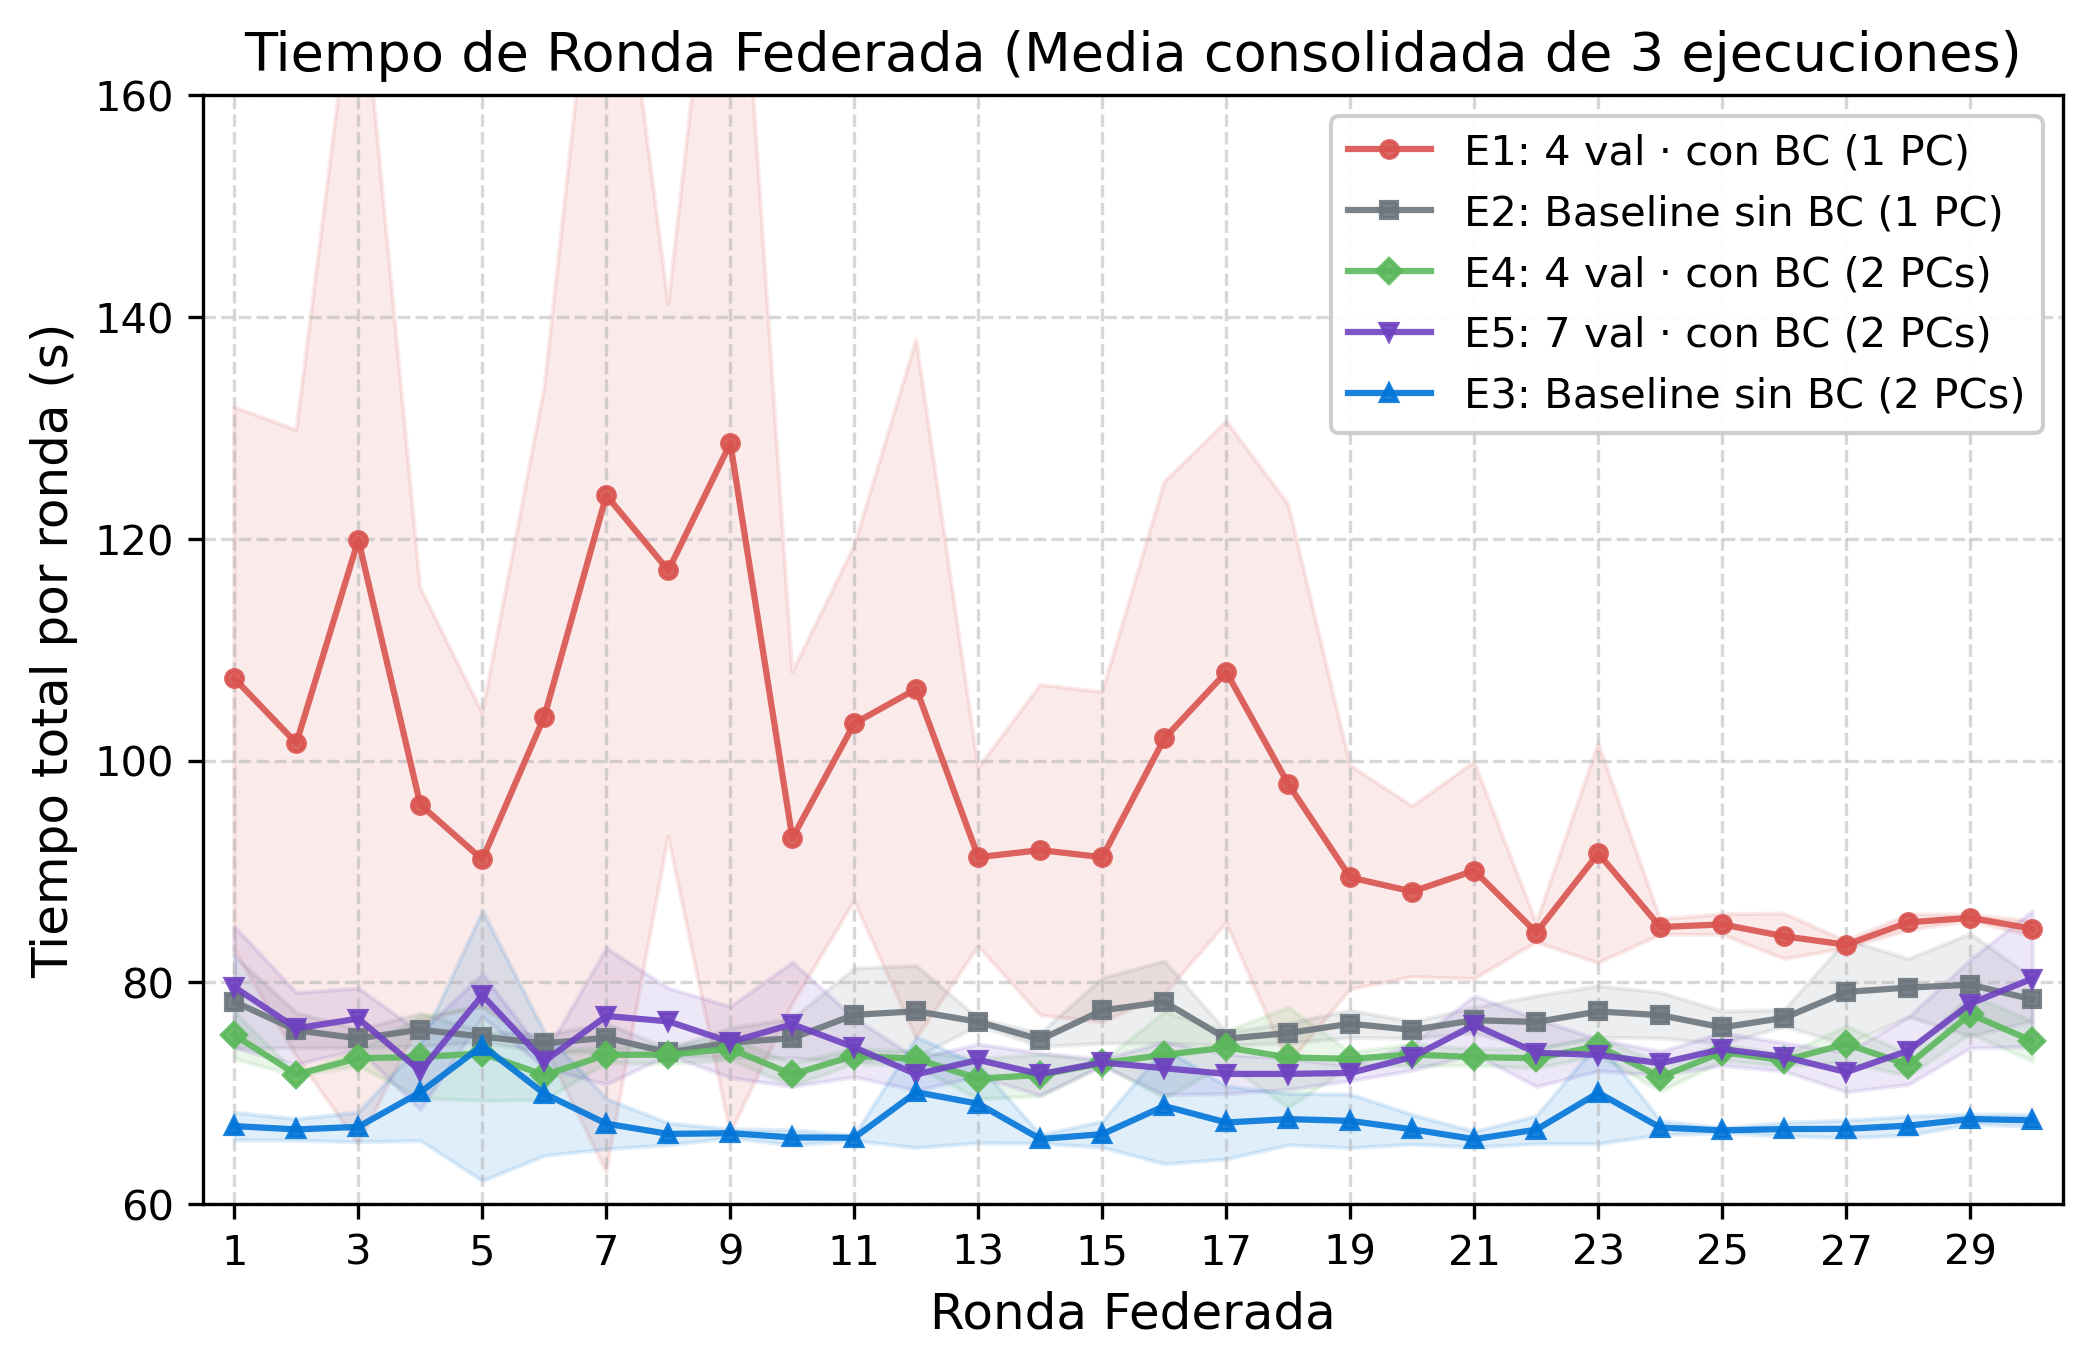
\includegraphics[width=\columnwidth]{figuras/tiempo_ronda_todas.png}
    \caption{Comparativa del tiempo de ciclo en clientes ($T_{\text{client}}$) a lo largo de las rondas en las cinco configuraciones experimentales.}
    \label{fig:tiempo_todas}
\end{figure}

El análisis multiejecución revela diferencias clave en la estabilidad de cada entorno. En la configuración local $E_1$, la dispersión inter-ejecución entre las medias de las tres repeticiones es de $\sigma_{\text{runs}} = 20{,}01$~s ($SE = 11{,}55$~s), registrando una dispersión longitudinal acumulada a lo largo de las 90 rondas de $\sigma_{\text{pool}} = 27{,}64$~s. Esta mayor variabilidad se debe a que, en la primera ejecución en monomáquina, los procesos de entrenamiento convolucional compitieron directamente en CPU y memoria con los ocho contenedores de Docker que soportaban los nodos de Besu y el daemon de IPFS. Por el contrario, en el entorno distribuido ($E_4$ y $E_5$), la variabilidad inter-ejecución se reduce drásticamente ($\sigma_{\text{runs}} \in [0{,}54, 1{,}28]$~s y $SE \le 0{,}74$~s; con dispersiones longitudinales contenidas en $\sigma_{\text{pool}} \le 3{,}92$~s), demostrando una gran estabilidad y reproducibilidad operativa. Por este motivo, se adopta la \textbf{mediana} como métrica central para aislar el comportamiento intrínseco del sistema frente a fluctuaciones externas.

\subsection{Sobrecoste Temporal Aislado de la Capa Blockchain}
Para cuantificar con exactitud el coste temporal impuesto por la serialización de tensores, la publicación en IPFS, la firma ECDSA y el consenso IBFT~2.0, se comparan las configuraciones equivalentes con y sin capa de seguridad (Figura~\ref{fig:coste_bc}):
\begin{itemize}
    \item \textbf{Escenario Monomáquina ($E_1$ vs. $E_2$)}: El tiempo mediano pasa de 75,70~s a 85,42~s, representando un sobrecoste de \textbf{+9,72~s (+12,8\%)}.
    \item \textbf{Escenario Distribuido ($E_3$ vs. $E_4$)}: El tiempo mediano se incrementa de 66,62~s a 72,96~s, lo que supone una sobrecarga de tan solo \textbf{+6,34~s (+9,5\%)}.
\end{itemize}

\begin{figure}[H]
    \centering
    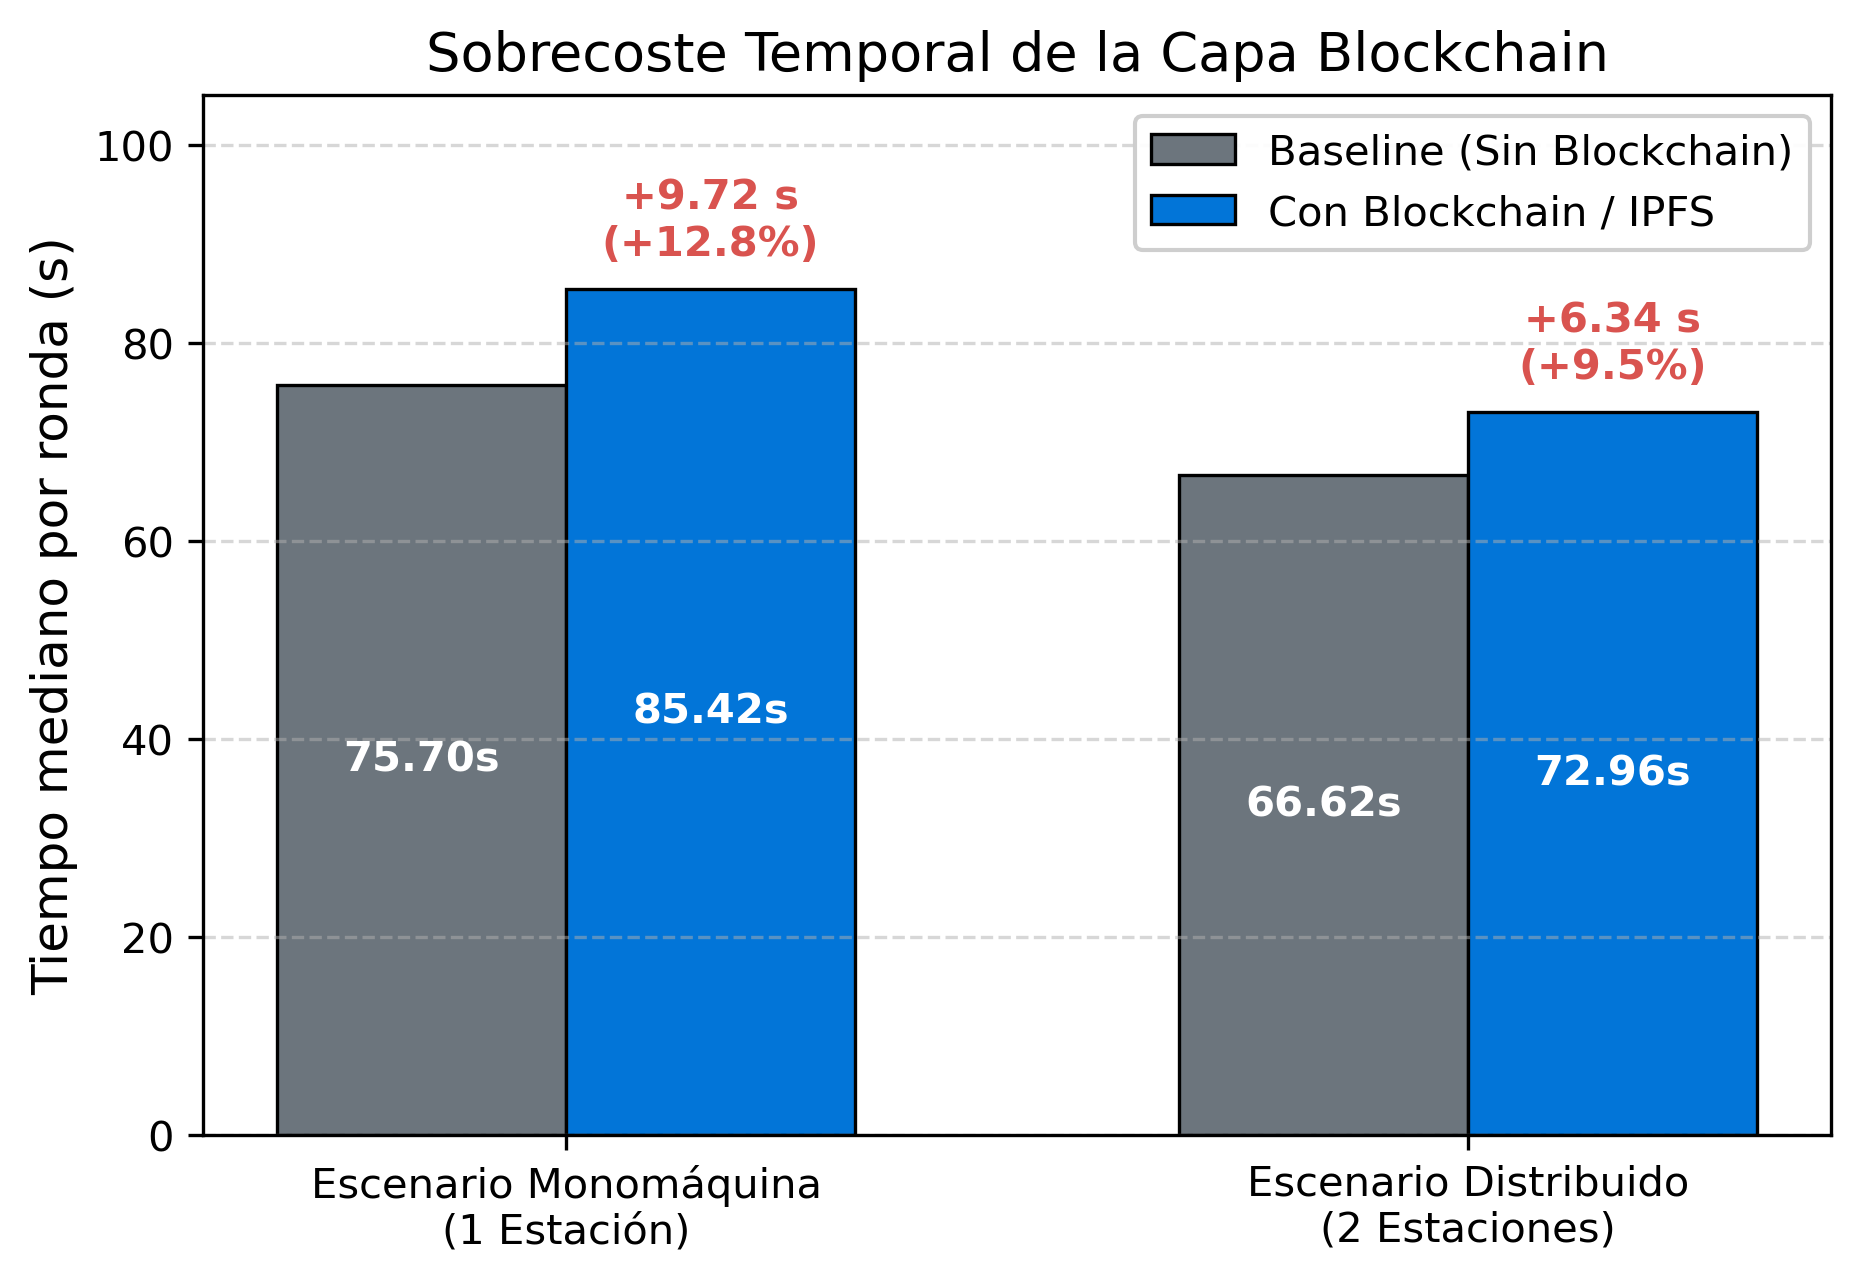
\includegraphics[width=\columnwidth]{figuras/coste_blockchain.png}
    \caption{Sobrecoste temporal inducido por la integración de la Blockchain en entornos local y distribuido.}
    \label{fig:coste_bc}
\end{figure}

Este hallazgo es de especial trascendencia para aplicaciones vehiculares y de borde: al desacoplar el entrenamiento de los clientes en una estación independiente, el impacto de la capa de auditoría e inmutabilidad se sitúa por debajo del 10\%. Una penalización de apenas 6 segundos por ronda resulta ampliamente asumible frente al beneficio de contar con un registro descentralizado inmutable y auditable.

\subsection{Efecto de la Distribución Física y Desglose por Fases}
La comparación entre la arquitectura monomáquina y distribuida demuestra que la separación física de roles optimiza el rendimiento global (Figura~\ref{fig:coste_dist}): el tiempo de ronda se reduce tanto en el baseline sin Blockchain (de 75,70~s a 66,62~s; un descenso de -12,0\%) como con Blockchain (de 85,42~s a 72,96~s; una reducción de -14,6\%).

\begin{figure}[H]
    \centering
    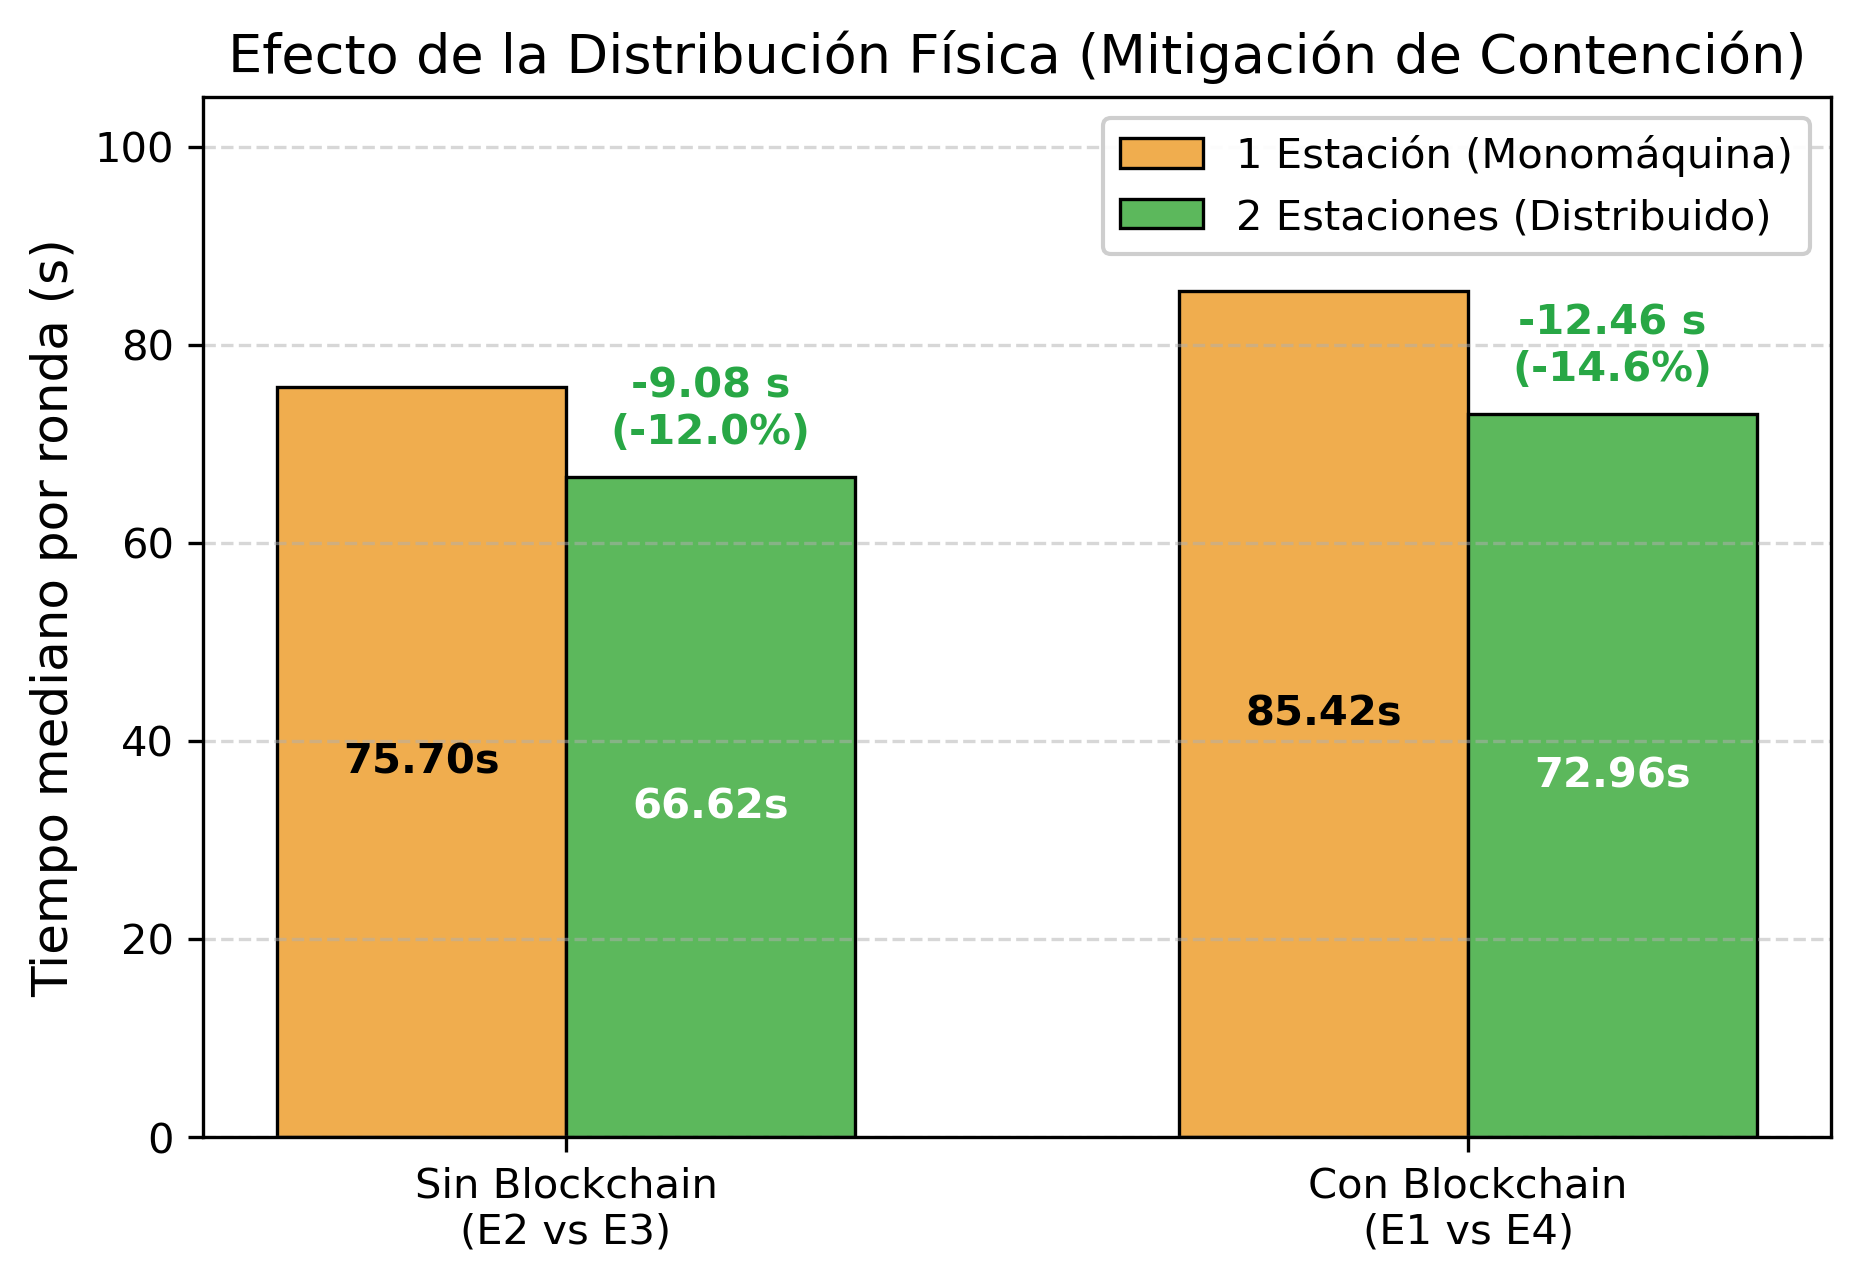
\includegraphics[width=\columnwidth]{figuras/coste_distribucion.png}
    \caption{Efecto de la distribución física de nodos sobre el tiempo de ciclo: mitigación de cuellos de botella de CPU/memoria.}
    \label{fig:coste_dist}
\end{figure}

Para explicar rigurosamente este comportamiento, la Tabla~\ref{tab:desglose_fases} descompone la latencia media de cada fase interna del ciclo federado tanto en los clientes (Estación 2) como en el servidor (Estación 1), evidenciando la correspondencia con las métricas agregadas de la Tabla~\ref{tab:tiempos_resumen}.

\begin{table}[H]
\centering
\caption{Desglose fino de la latencia media por fase en cliente ($T_{\text{client}}$) y servidor ($T_{\text{server}}$) (segundos).}
\label{tab:desglose_fases}
\resizebox{\columnwidth}{!}{%
\begin{tabular}{@{}lcccc|cccc@{}}
\toprule
& \multicolumn{4}{c|}{\textbf{Fases Cliente (Estación 2)}} & \multicolumn{4}{c}{\textbf{Fases Servidor (Estación 1)}} \\
\cmidrule(lr){2-5} \cmidrule(lr){6-9}
\textbf{Exp.} & \textbf{Train} & \textbf{Verif.} & \textbf{IPFS} & \textbf{Tx Besu} & \textbf{Espera} & \textbf{Verif.} & \textbf{FedAvg} & \textbf{Bloque} \\
\midrule
$E_1$ & 94,08 & 0,08 & 0,06 & 2,85 & 98,16 & 0,05 & 0,0065 & 5,14 \\
$E_2$ & 76,45 & 0,00 & 0,00 & 0,00 & 77,02 & 0,00 & 0,0040 & 0,00 \\
\midrule
$E_3$ & 67,62 & 0,00 & 0,00 & 0,00 & 71,07 & 0,00 & 0,0036 & 0,00 \\
$E_4$ & 66,22 & 1,68 & 2,43 & 2,84 & 79,54 & 0,06 & 0,0047 & 2,89 \\
$E_5$ & 65,40 & 1,91 & 3,93 & 2,94 & 82,63 & 0,06 & 0,0079 & 2,99 \\
\bottomrule
\end{tabular}%
}
\end{table}

Los datos de la Tabla~\ref{tab:desglose_fases} confirman tres principios fundamentales:
\begin{enumerate}
    \item \textbf{Desacoplamiento de cómputo:} En las configuraciones distribuidas ($E_3$, $E_4$, $E_5$), el tiempo dedicado exclusivamente a la optimización neuronal con PyTorch se mantiene estrictamente invariante ($\sim 65,4\text{--}67,6$~s), evitando la contención de recursos observada en $E_1$ ($94,08$~s).
    \item \textbf{Sobrecarga de red y verificación acotadas:} La verificación remota vía RPC ($1,68\text{--}1,91$~s en cliente y $\sim 5$~ms en servidor), la transferencia IPFS ($2,43\text{--}3,93$~s) y el cómputo in-memory del multihash de pesos en el servidor ($\sim 52$~ms en el código final, $<0{,}08\%$ del ciclo) añaden una latencia mínima, mientras que el cálculo de FedAvg es despreciable ($< 8$~ms).
    \item \textbf{Correspondencia entre métricas ($T_{\text{client}}$ y $T_{\text{server}}$):} La suma de las cuatro fases locales del cliente (\textit{Train} + \textit{Verif.} + \textit{IPFS} + \textit{Tx Besu}) totaliza con exactitud el tiempo de ciclo reportado en la Tabla~\ref{tab:tiempos_resumen} (por ejemplo, en $E_4$: $66{,}22 + 1{,}68 + 2{,}43 + 2{,}84 = 73{,}17$~s, en plena coherencia con la media de $73{,}29$~s). Paralelamente, la perspectiva del servidor refleja la duración global de la ronda en el agregador ($T_{\text{server}}$), donde el servidor aguarda la concurrencia de todos los clientes (\textit{Espera}, $79{,}54$~s) y añade la confirmación del nuevo modelo consolidado en la cadena (\textit{Bloque}, $2{,}89$~s), totalizando una latencia extremo a extremo de $\approx 82{,}49$~s.
\end{enumerate}

\subsection{Escalado de Consenso Bizantino IBFT 2.0 (4 frente a 7 Validadores)}
En redes permisionadas, la tolerancia a fallos bizantinos sigue el principio $N \ge 3f + 1$, donde $N$ es el conjunto de validadores y $f$ el número máximo de nodos bizantinos o caídos:
\begin{itemize}
    \item Red de 4 validadores ($E_4$): tolera $f=1$ fallo; quórum de firmas necesario $2f+1 = 3$.
    \item Red de 7 validadores ($E_5$): tolera $f=2$ fallos; quórum de firmas necesario $2f+1 = 5$.
\end{itemize}

Al comparar $E_4$ con $E_5$, la mediana por ronda apenas varía de 72,96~s a 73,35~s (+0,39~s), lo que evidencia que la latencia global del ciclo sigue dominada por el entrenamiento local.

\begin{figure}[H]
    \centering
    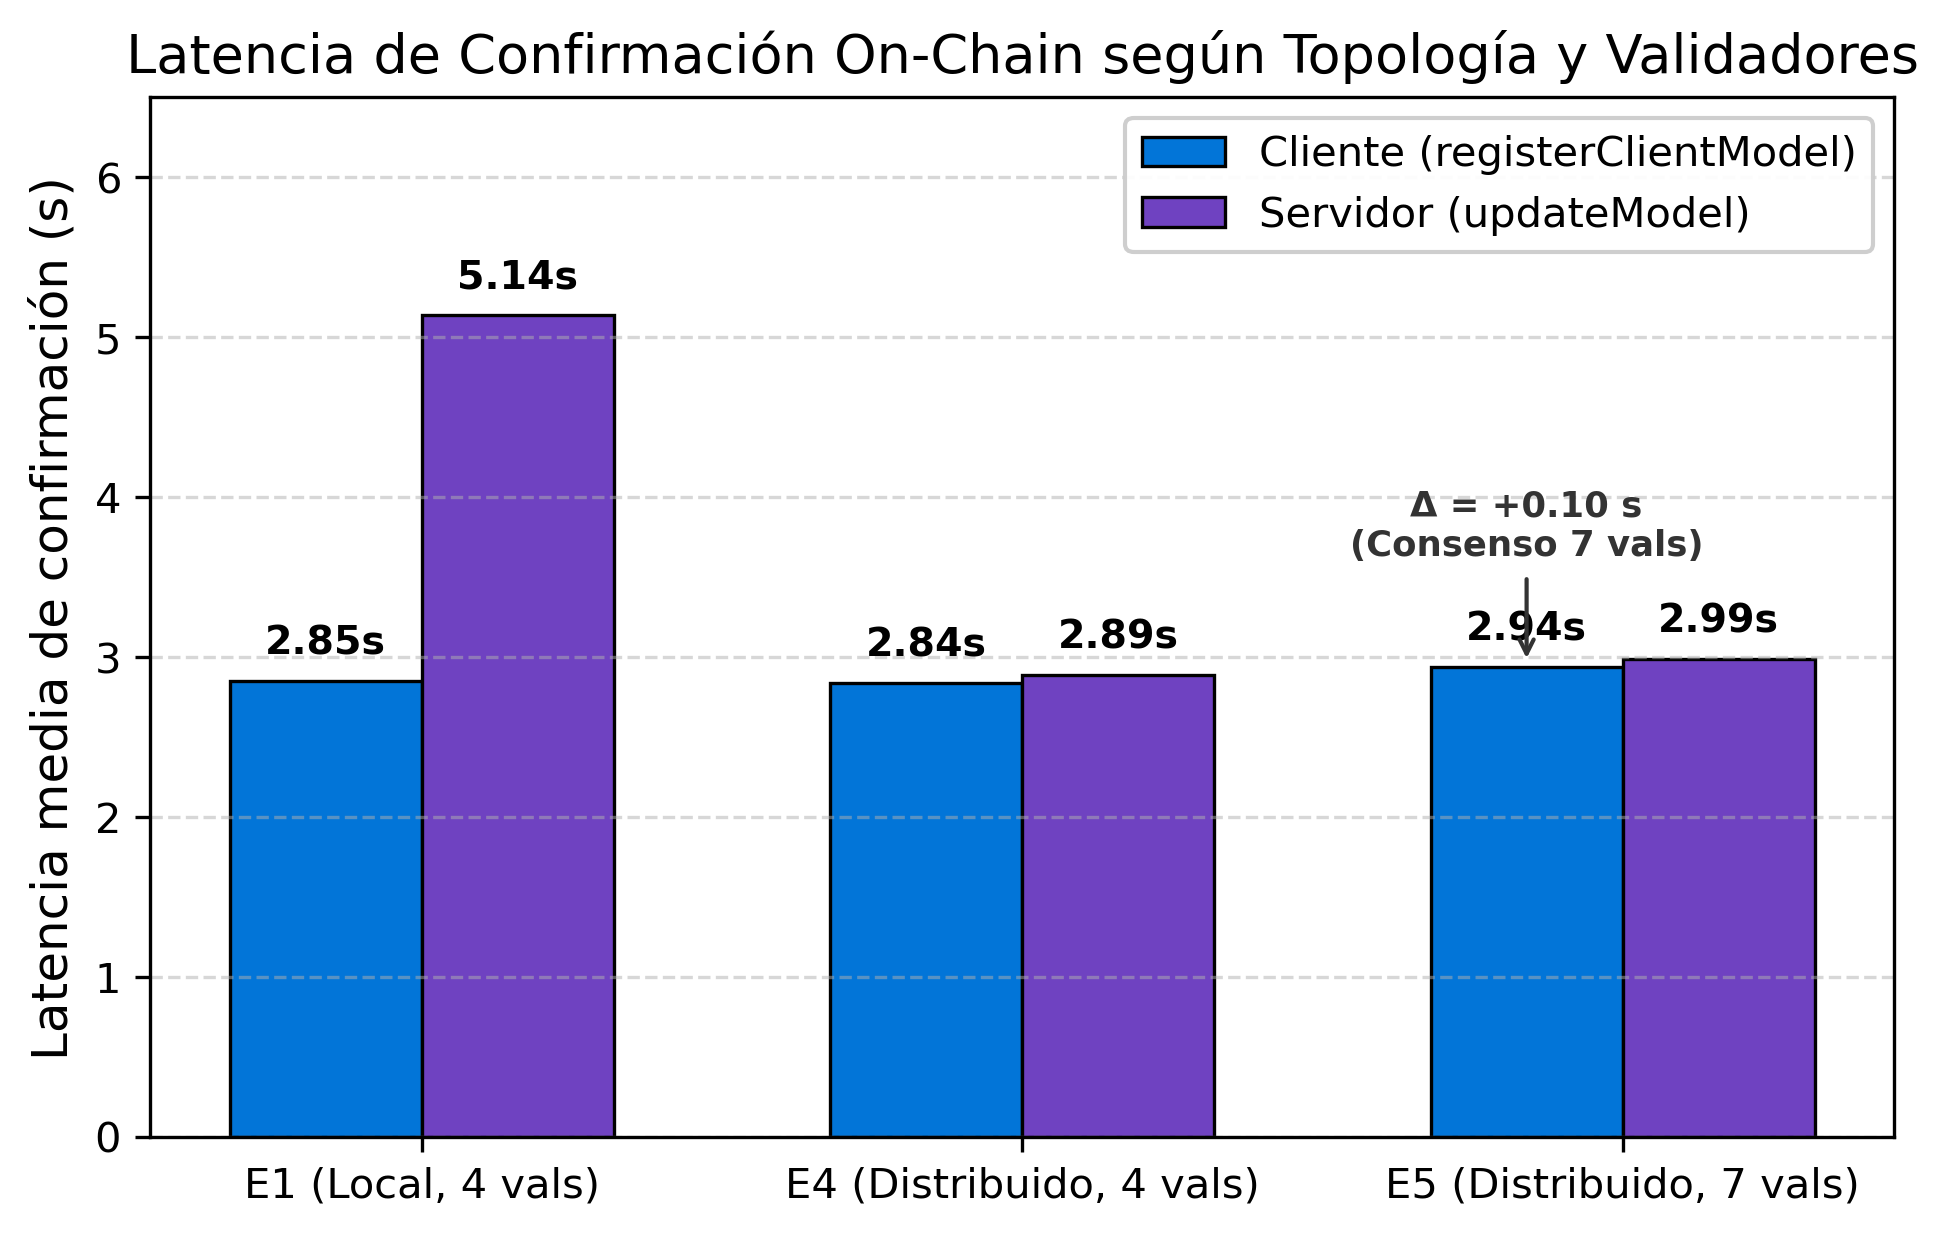
\includegraphics[width=\columnwidth]{figuras/tiempo_confirmacion.png}
    \caption{Tiempo medio de confirmación de transacción según topología y número de validadores en Hyperledger Besu.}
    \label{fig:tiempo_confirmacion}
\end{figure}

Al aislar específicamente el \textbf{tiempo de confirmación de las transacciones on-chain} (Figura~\ref{fig:tiempo_confirmacion}), la complejidad de intercambio de mensajes del algoritmo IBFT~2.0 ($\mathcal{O}(N^2)$ en fases \textit{Prepare} y \textit{Commit}) se manifiesta de manera clara:
\begin{itemize}
    \item Transacción del cliente (\texttt{registerClientModel}): la latencia media pasa de 2,84~s en $E_4$ a 2,94~s en $E_5$ (+0,10~s).
    \item Transacción del servidor (\texttt{updateModel}): la latencia pasa de 2,89~s en $E_4$ a 2,99~s en $E_5$ (+0,10~s).
\end{itemize}
Este incremento simétrico de 100~ms confirma experimentalmente que ampliar la resiliencia bizantina del consorcio de 1 a 2 nodos fallidos no compromete la viabilidad temporal del sistema.

\subsection{Robustez Adversarial y Verificación Experimental de Ataques}
\label{subsec:ataques}
Para validar empíricamente que la arquitectura no solo registra transacciones en condiciones nominales, sino que neutraliza activamente vectores de ataque reales, se implementó una batería de ensayos adversariales controlados en el módulo \texttt{test\_verificacion.py}. El objetivo es evaluar el comportamiento del sistema ante las dos principales amenazas bizantinas en aprendizaje federado no confiable: un servidor central comprometido (ataque descendente) y un nodo participante envenenador (ataque ascendente).

\subsubsection{Prueba 1: Verificación Descendente (Servidor Adulterado frente a Cliente Edge)}
\label{subsubsec:ataque_descendente}
En un entorno federado no confiable, la distribución descendente de parámetros expone a los clientes a dos vectores de riesgo principales: la alteración de los tensores en tránsito por intermediarios de red (\textit{Man-in-the-Middle}) y la bifurcación maliciosa o equivocación del servidor (\textit{server equivocation}), donde un agregador deshonesto intenta distribuir modelos globales distintos o sesgados selectivamente a participantes específicos. Cabe destacar que la validez del modelo global on-chain queda estrictamente acotada a la entidad autorizada gracias al modificador de control de acceso \texttt{onlyServer} en el contrato \texttt{FLRegistry}, el cual revierte cualquier intento de registro por cuentas no autorizadas. Así, la rutina de verificación descendente implementada en el cliente protege de forma autónoma frente a discrepancias entre los pesos recibidos por gRPC y el compromiso sellado institucionalmente en la Blockchain:
\begin{enumerate}
    \item \textbf{Generación y Sellado Oficial:} El servidor legítimo instancia el modelo base \texttt{NetCliente}, serializa los tensores mediante \texttt{pickle.dumps} y los publica en el daemon IPFS local a través del endpoint \texttt{/api/v0/add?pin=false}, obteniendo el CID oficial \texttt{QmQTpgejdzh...}. A continuación, el servidor emite una transacción firmada en la EVM invocando \texttt{updateModel(round, cid\_oficial)} desde su cuenta autorizada (\texttt{0xfe3b55...}), quedando el compromiso criptográfico sellado en el \textbf{Bloque~80}.
    \item \textbf{Inyección Adversarial y Simulación de Discrepancia:} Se emula un escenario adversarial donde se perturban los parámetros transmitidos al cliente inyectando ruido aditivo ($\mathbf{w}_{\text{cand}} = \mathbf{w}_{\text{oficial}} + 0{,}5$) y remitiendo este vector corrupto vía gRPC (simulando alteración en tránsito o un intento del servidor de suministrar una versión discrepante del modelo oficial).
    \item \textbf{Comprobación Cruzada y Aborto Inmediato:} Al recibir la orden de entrenamiento, el cliente edge invoca la función de solo lectura \texttt{getLastModel()} en el Smart Contract mediante una llamada JSON-RPC para recuperar el CID sellado on-chain. Con este identificador descarga de forma paralela el artefacto binario de referencia desde la pasarela IPFS (\texttt{/ipfs/<CID>}) y ejecuta una comparación numérica tensorial elemento a elemento con cota de tolerancia de coma flotante (\texttt{np.allclose(p\_recibido, p\_ipfs, atol=1e-7)}).
\end{enumerate}

\begin{center}
\small
\fbox{
\begin{minipage}{0.95\columnwidth}
\textbf{Algoritmo 1. Verificación Descendente en el Cliente Edge}
\begin{enumerate}
    \item \textbf{Entrada:} Pesos candidatos $\mathbf{w}_{\text{cand}}$ remitidos vía gRPC por el servidor.
    \item Consultar contrato en Besu: $\text{CID}_{\text{onchain}} \leftarrow \texttt{FLRegistry.getLastModel().cid}$
    \item Descargar binario de IPFS: $\mathbf{w}_{\text{ipfs}} \leftarrow \texttt{IPFS.get}(\text{CID}_{\text{onchain}})$
    \item \textbf{Si} $\exists l : \|\mathbf{w}_{\text{cand}, l} - \mathbf{w}_{\text{ipfs}, l}\|_{\infty} > \epsilon$ \textbf{entonces}
    \begin{itemize}
        \item Registrar alerta: \textit{«Discrepancia detectada en pesos recibidos»}
        \item \textbf{ABORTAR} ronda localmente (bloquear backpropagation)
    \end{itemize}
    \item \textbf{Si no:} Aceptar $\mathbf{w}_{\text{cand}}$ y proseguir con el entrenamiento local.
\end{enumerate}
\end{minipage}
}
\end{center}

La Figura~\ref{fig:log_ataque_descendente} ilustra la telemetría real en tiempo de ejecución capturada en la consola del cliente. El proceso íntegro de consulta RPC a Besu, descarga y cotejo tensorial insumió tan solo \textbf{0{,}1486~segundos} (149~ms). Al constatar la discrepancia, el cliente detuvo de forma inmediata la ejecución, impidiendo la contaminación de su modelo local y salvaguardando los datos de entrenamiento privados del vehículo.

\begin{figure}[H]
    \centering
    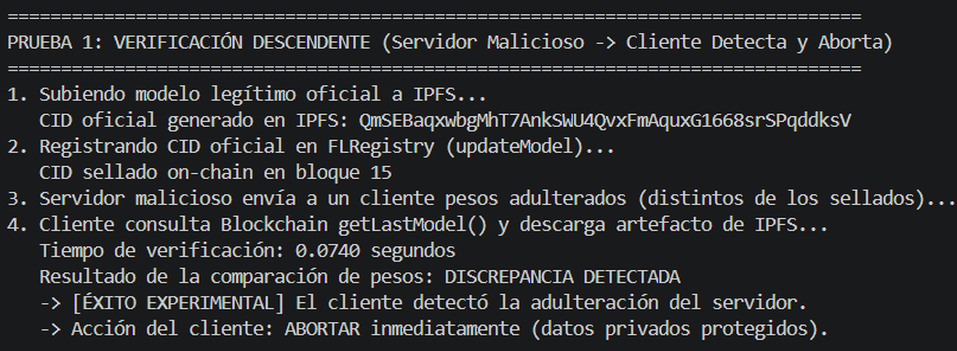
\includegraphics[width=\columnwidth]{figuras/logs_deteccion_ataque_descendent.png}
    \caption{Prueba 1: Registro de consola del nodo cliente detectando la adulteración del modelo frente al CID oficial sellado en el bloque}
    \label{fig:log_ataque_descendente}
\end{figure}

Por su parte, la Figura~\ref{fig:bloque_80_audit} aporta la evidencia inmutable en la cadena de bloques, capturada desde el explorador de la red Hyperledger Besu. En ella se observa el sellado de la transacción \texttt{updateModel} en el \textbf{Bloque~80}, emitida por la dirección del servidor (\texttt{0xfe3b557e...}) con hash criptográfico \texttt{0x973b0b...} y un consumo de gas de 167.460 (límite 500.000). Esta correspondencia unívoca entre el bloque minado y la verificación del cliente valida la consistencia del protocolo.

\begin{figure}[H]
    \centering
    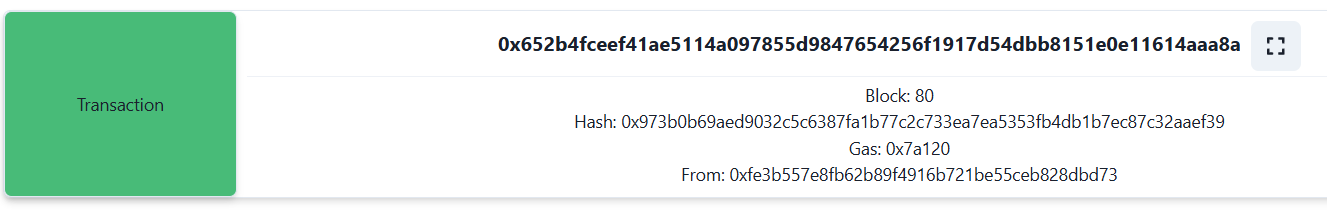
\includegraphics[width=\columnwidth]{figuras/auditoria_grafana_bloque_80.png}
    \caption{Prueba 1: Confirmación en Hyperledger Besu del bloque 80, registrando la transacción oficial \texttt{updateModel} emitida por el servidor agregador.}
    \label{fig:bloque_80_audit}
\end{figure}

\subsubsection{Prueba 2: Verificación Ascendente (Cliente Envenenador frente a Servidor Agregador)}
\label{subsubsec:ataque_ascendente}
La segunda vulnerabilidad crítica consiste en la inyección de gradientes o pesos corruptos por parte de un nodo cliente malicioso (\textit{model poisoning}). Para neutralizarla de raíz, el servidor no se limita a cotejar identificadores, sino que valida de forma cruzada la correspondencia biunívoca entre la carga útil recibida en memoria y el registro inmutable on-chain:
\begin{enumerate}
    \item \textbf{Registro Legítimo On-Chain:} El nodo cliente honesto (cuenta 3, dirección \texttt{0xf17f52...}) publica sus pesos en IPFS y emite una transacción firmada con su clave privada invocando \texttt{registerClientModel}\allowbreak\texttt{(round, cid\_legitimo)}, la cual queda consolidada por los validadores en el \textbf{Bloque~81}.
    \item \textbf{Inyección Adversarial:} Se evalúa el comportamiento ante un intento de inyección donde se remite al servidor una actualización cuyos parámetros o metadatos no coinciden con el compromiso sellado on-chain (emulando tanto el envío de un identificador malicioso \texttt{QmClientFraud...} como el envío de pesos envenenados no correspondientes con el CID registrado).
    \item \textbf{Auditoría Criptográfica y Descarte en FedAvg:} Antes de procesar la agregación matricial de la ronda, el servidor calcula el hash de los tensores recibidos en memoria ($\text{CID}_{\text{calc}}^{(k)}$) y ejecuta una llamada de solo lectura JSON-RPC \texttt{getClientModel(round, address)} sobre el contrato \texttt{FLRegistry} para obtener $\text{CID}_{\text{onchain}}^{(k)}$. Al constatar la discrepancia, la contribución es excluida de forma preventiva.
\end{enumerate}

\begin{center}
\small
\fbox{
\begin{minipage}{0.95\columnwidth}
\textbf{Algoritmo 2. Auditoría Criptográfica y RPC Ascendente en el Servidor Agregador}
\begin{enumerate}
    \item \textbf{Entrada:} Pesos $\mathbf{w}_k^{(t)}$ e identificador $\text{CID}_{\text{rep}}^{(k)}$ reportados por el cliente $k$ con dirección $\text{addr}_k$.
    \item Computar hash de los pesos recibidos: \\
    $\text{CID}_{\text{calc}}^{(k)} \leftarrow \text{Hash}(\mathbf{w}_k^{(t)})$
    \item Consultar registro del cliente en Besu: \\
    $\text{CID}_{\text{onchain}}^{(k)} \leftarrow \texttt{getClientModel}(t, \text{addr}_k)$
    \item \textbf{Si} $\text{CID}_{\text{rep}}^{(k)} \neq \text{CID}_{\text{onchain}}^{(k)}$ \textbf{o} $\text{CID}_{\text{calc}}^{(k)} \neq \text{CID}_{\text{onchain}}^{(k)}$ \textbf{entonces}
    \begin{itemize}
        \item Registrar alerta: \textit{«Discrepancia detectada / Inyección no autenticada»}
        \item \textbf{DESCARTAR} contribución del cliente $k$ del pool de FedAvg
    \end{itemize}
    \item \textbf{Si no:} Incorporar pesos $\mathbf{w}_k^{(t)}$ en la agregación global.
\end{enumerate}
\end{minipage}
}
\end{center}

La Figura~\ref{fig:log_ataque_ascendente} documenta la salida en terminal del servidor agregador. La llamada JSON-RPC a la EVM tomó únicamente \textbf{0{,}0309~segundos} (31~ms). Al constatar que el CID no coincidía con la transacción firmada del cliente, el servidor excluyó al participante de la agregación de forma inmediata, preservando la convergencia y la integridad del modelo global.

\begin{figure}[H]
    \centering
    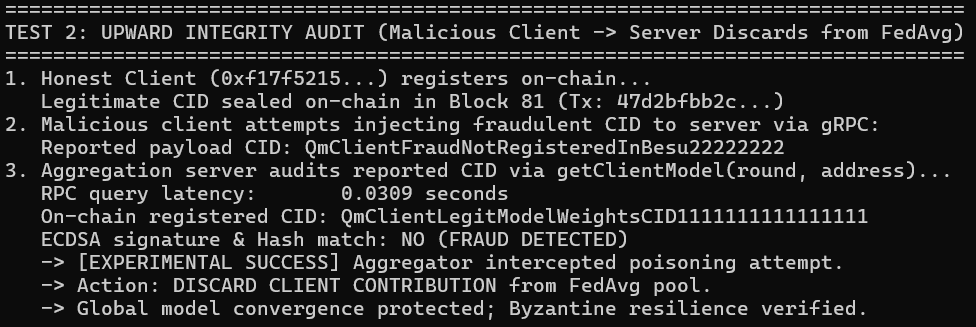
\includegraphics[width=\columnwidth]{figuras/logs_deteccion_ataque_ascendente.png}
    \caption{Prueba 2: Registro de consola del servidor agregador auditando vía RPC el CID del cliente y descartando la contribución fraudulenta}
    \label{fig:log_ataque_ascendente}
\end{figure}

La Figura~\ref{fig:bloque_81_audit} muestra el recibo del \textbf{Bloque~81} en el explorador Besu, donde consta la transacción \texttt{registerClientModel} emitida por la cuenta del cliente (\texttt{0xf17f5215...}) con hash \texttt{0x347899f...} y un consumo de gas de 160.200 (límite 200.000). Dado que el atacante remitió un CID ajeno al sellado en dicho bloque, la verificación cruzada interceptó la inyección adversarial gracias a la resistencia a colisiones de la función hash SHA-256 subyacente al CID de IPFS.

\begin{figure}[H]
    \centering
    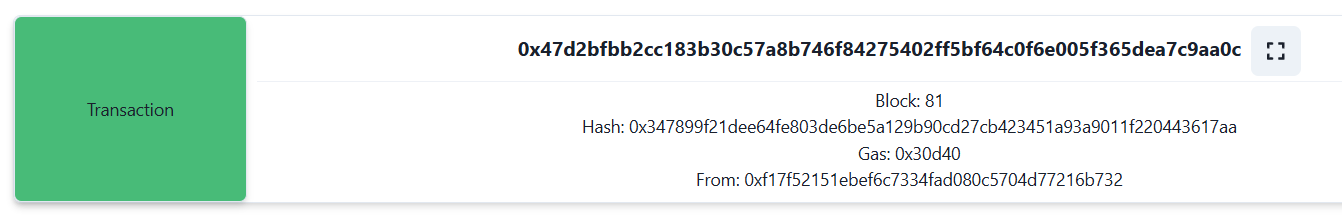
\includegraphics[width=\columnwidth]{figuras/auditoria_grafana_bloque_81.png}
    \caption{Prueba 2: Confirmación forense en Hyperledger Besu del bloque 81, registrando la transacción legítima \texttt{registerClientModel} del nodo cliente.}
    \label{fig:bloque_81_audit}
\end{figure}

\subsubsection{Prueba 3: Auditoría Ex-Post y Verificabilidad Independiente de FedAvg}
\label{subsubsec:auditoria_expost_eval}
Para validar la tercera garantía de integridad formalizada en la Sección~\ref{subsec:auditoria_fedavg}, se evaluó experimentalmente la capacidad de un agente auditor externo o regulador para fiscalizar \textit{a posteriori} y de forma autónoma la fidelidad de la agregación ejecutada por el servidor central. Esta prueba permite auditar matemáticamente si el agregador ha respetado la regla canónica de agregación sin introducir sesgos, omisiones ni alteraciones paramétricas no autorizadas.

El ensayo se ejecutó sobre la Ronda~2 de un entrenamiento real de aprendizaje federado con dos clientes edge concurrentes conectados a la red Hyperledger Besu (contrato \texttt{0x42699A76...}) e IPFS. La Tabla~\ref{tab:trazabilidad_ronda2} sintetiza la cadena de custodia completa de dicha ronda, correlacionando de forma unívoca las cuentas emisoras, las transacciones selladas en los bloques consecutivos 73, 74 y 75, los identificadores multihash IPFS y las latencias registradas.

\begin{table}[H]
\centering
\caption{Cadena de custodia y trazabilidad cruzada on-chain/IPFS durante la Ronda 2 y su fiscalización ex-post.}
\label{tab:trazabilidad_ronda2}
\resizebox{\columnwidth}{!}{%
\begin{tabular}{@{}lcccccc@{}}
\toprule
\textbf{Entidad} & \textbf{Dirección Ethereum} & \textbf{Evento / Método} & \textbf{Bloque Besu} & \textbf{Latencia} & \textbf{CID IPFS} & \textbf{Estado / Resultado} \\
\midrule
Cliente 3 & \texttt{0xf17f5215...} & \texttt{registerClientModel} & Bloque 73 & 0,886 s & \texttt{QmS5ViVf...} & Confirmado on-chain \\
Cliente 2 & \texttt{0x62730609...} & \texttt{registerClientModel} & Bloque 74 & 4,311 s & \texttt{QmNh3TLS...} & Confirmado on-chain \\
Servidor  & \texttt{0xfe3b557e...} & \texttt{updateModel} (FedAvg) & Bloque 75 & 4,709 s & \texttt{QmWF7tJ1...} & Modelo global sellado \\
\midrule
Auditor   & \textit{Externo (Off-chain)} & Reconstrucción FedAvg & Consulta 73--75 & 0,339 s & \texttt{QmWF7tJ1...} & \textbf{$\Delta = 0{,}000000$ (MATCH)} \\
\bottomrule
\end{tabular}%
}
\end{table}

El protocolo de auditoría operó conforme a las siguientes etapas:
\begin{enumerate}
    \item \textbf{Extracción e indexación on-chain:} De forma desacoplada y fuera de banda, el auditor identifica dinámicamente a los clientes participantes $\mathcal{K}_2$ consultando los registros de eventos \texttt{ModelUpdated} de la Ronda~2 en Besu (descubriendo las cuentas del Cliente~2 y Cliente~3) y recupera sus compromisos criptográficos sellados (\texttt{QmNh3TLS...} y \texttt{QmS5ViVf...}), junto con el modelo global reportado por el servidor (\texttt{QmWF7tJ1...}).
    \item \textbf{Descarga y reconstrucción determinista:} El auditor descarga los tres artefactos binarios desde la pasarela IPFS ($2{,}08$~MB por modelo, totalizando $6{,}24$~MB recuperados en $0{,}200$~s acumulados [$0{,}096$~s, $0{,}044$~s y $0{,}060$~s]) y ejecuta la agregación matricial canónica de FedAvg:
    \begin{equation}
    \mathbf{w}_{\text{recon}}^{(2)} = \frac{1}{2}\mathbf{w}_{\text{cli2}}^{(2)} + \frac{1}{2}\mathbf{w}_{\text{cli3}}^{(2)}
    \end{equation}
    generando el hash IPFS del modelo resultante mediante el algoritmo multihash SHA-256.
    \item \textbf{Verificación tensorial y criptográfica:} Se cotejan capa por capa los parámetros del modelo reconstruido frente al modelo global sellado por el servidor en el Bloque~75.
\end{enumerate}

\begin{figure}[H]
    \centering
    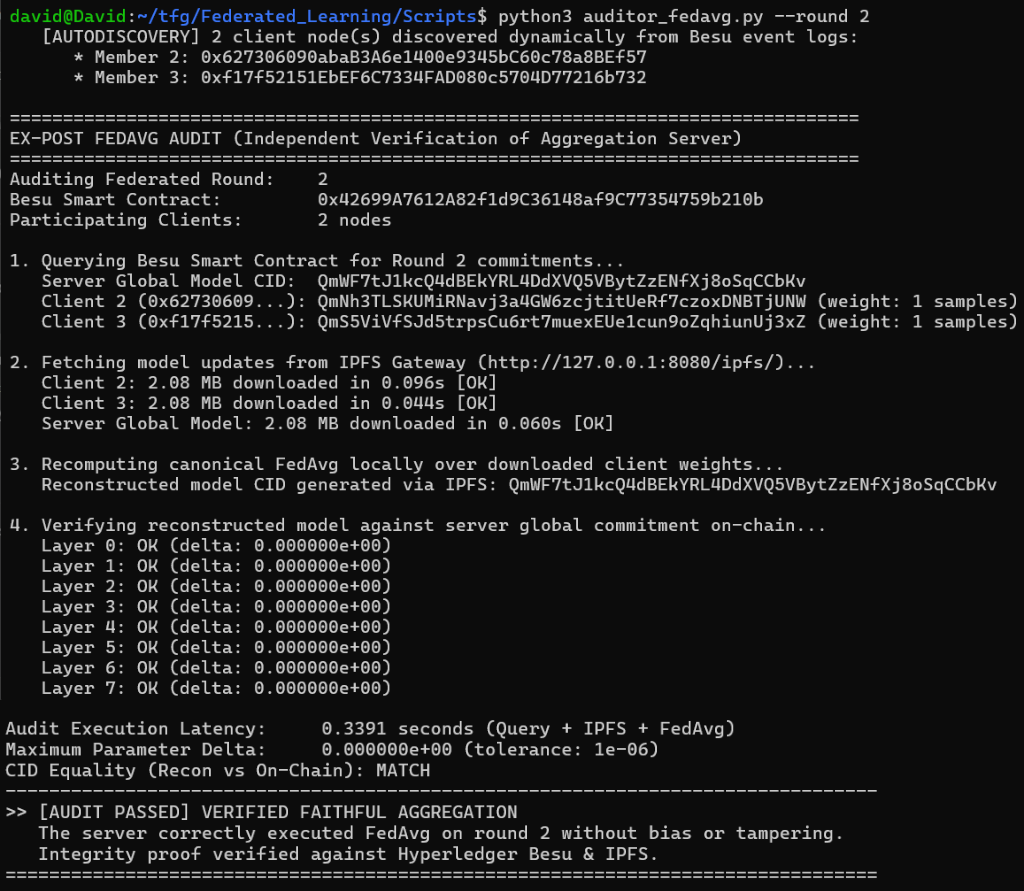
\includegraphics[width=\columnwidth]{figuras/logs_auditoria_expost_fedavg.png}
    \caption{Prueba 3: Registro de consola del auditor independiente reconstruyendo la agregación FedAvg de la Ronda 2 a partir de Besu e IPFS, verificando fidelidad estricta ($\Delta = 0{,}000000$) y coincidencia de CID.}
    \label{fig:log_auditoria_expost}
\end{figure}

\begin{table*}[t]
\centering
\caption{Validación experimental del marco de integridad y auditoría frente a escenarios de manipulación y verificación ex-post.}
\label{tab:resumen_ataques}
\resizebox{\textwidth}{!}{%
\renewcommand{\arraystretch}{1.2}
\begin{tabular}{@{}lcccc@{}}
\toprule
\textbf{Escenario de Prueba} & \textbf{Entidad Defensora / Auditora} & \textbf{Acción Preventiva / Resultado} & \textbf{Latencia} & \textbf{Integridad de Pesos} \\
\midrule
Manipulación en Tránsito / Servidor No Fidedigno & Cliente (Edge) & Intercepción determinista / Aborto preventivo & 0,1486 s & Sin contaminación local \\
Inyección No Autenticada / Cliente No Registrado & Servidor Agregador & Intercepción determinista / Descarte en FedAvg & 0,0309 s & Agregación preservada \\
Auditoría FedAvg Ex-Post & Auditor Independiente & Reconstrucción matemática / Verificación fidedigna & 0,3391 s & Fidelidad exacta ($\Delta = 0$, CID MATCH) \\
\bottomrule
\end{tabular}%
}
\end{table*}

Como refleja la telemetría en tiempo de ejecución capturada en la Figura~\ref{fig:log_auditoria_expost}, la auditoría integral (autodescubrimiento dinámico de participantes vía eventos Besu, consulta RPC de compromisos, descarga de 6,24~MB de IPFS, reconstrucción tensorial y verificación exhaustiva de las 8 capas de la red convolucional) requirió únicamente \textbf{0,3391~segundos}. La discrepancia paramétrica en todas las capas convolucionales y completamente conexas fue estrictamente nula ($\Delta = 0{,}000000\text{e}+00$), derivando en un identificador CID idéntico carácter a carácter al registrado en el Bloque~75 (\texttt{CID Equality: MATCH}), ratificando de forma incontrovertible la concordancia de la agregación.

Asimismo, se evaluó la sensibilidad del mecanismo activando el modo adversarial simulado (\texttt{--simulate-tampering}). Al inyectar una perturbación aditiva deliberada de $+0{,}1$ en los pesos del servidor, el auditor detectó la desviación de forma instantánea en tan solo \textbf{0,1805~segundos} ($\Delta = 1{,}000000\text{e}-01$), registrando una alerta formal de discrepancia no conforme (\texttt{AUDIT FAILED: DISCREPANCY DETECTED}).

\subsubsection{Síntesis de Validación y Alcance de Seguridad}
La Tabla~\ref{tab:resumen_ataques} sintetiza las métricas cuantitativas obtenidas a lo largo de las tres pruebas experimentales de integridad y auditoría.

Estos ensayos constituyen una validación funcional determinista de las primitivas de intercepción criptográfica implementadas en el marco: ante una alteración de los parámetros en tránsito o la ausencia de un compromiso inmutable previamente sellado y firmado en la cadena, el protocolo intercepta la anomalía de manera determinista con tiempos de respuesta en torno a la décima de segundo (149~ms en el cliente, 31~ms en el servidor y $\approx 200$~ms en la auditoría ex-post de FedAvg), impidiendo que los pesos discordantes contaminen los cómputos locales o globales.

Tal como se formalizó en el modelo de amenazas (Sección~\ref{subsec:modelo_amenazas}), conviene remarcar los límites operacionales de este esquema defensivo: la doble verificación en cadena actúa con eficacia contra la adulteración directa de parámetros en tránsito (\textit{tampering}), la emisión no autorizada a nombre de terceros mediante autenticación asimétrica ECDSA y la inyección de modelos disidentes no respaldados on-chain. No obstante, si un nodo malicioso genera una actualización perjudicial mediante manipulación local de sus datos de entrenamiento (\textit{data poisoning} o \textit{label flipping})~\cite{tolpegin2020data} y la firma legítimamente con su clave privada en Besu, el compromiso criptográfico coincidirá formalmente aunque la semántica del modelo esté contaminada. La neutralización de esta tipología de ataques semánticos requiere complementar la trazabilidad con filtros de agregación estadística bizantina (como Krum~\cite{blanchard2017byzantine}, Median o Trimmed-Mean) o mediante la auditoría ex-post de las contribuciones registradas posibilitada por nuestro diseño (Sección~\ref{subsec:auditoria_fedavg}).

\subsection{Consumo y Previsibilidad del Gas en la EVM}
La Figura~\ref{fig:consumo_gas} ilustra el consumo de gas computacional de las operaciones registradas a lo largo de las rondas.

\begin{figure}[H]
    \centering
    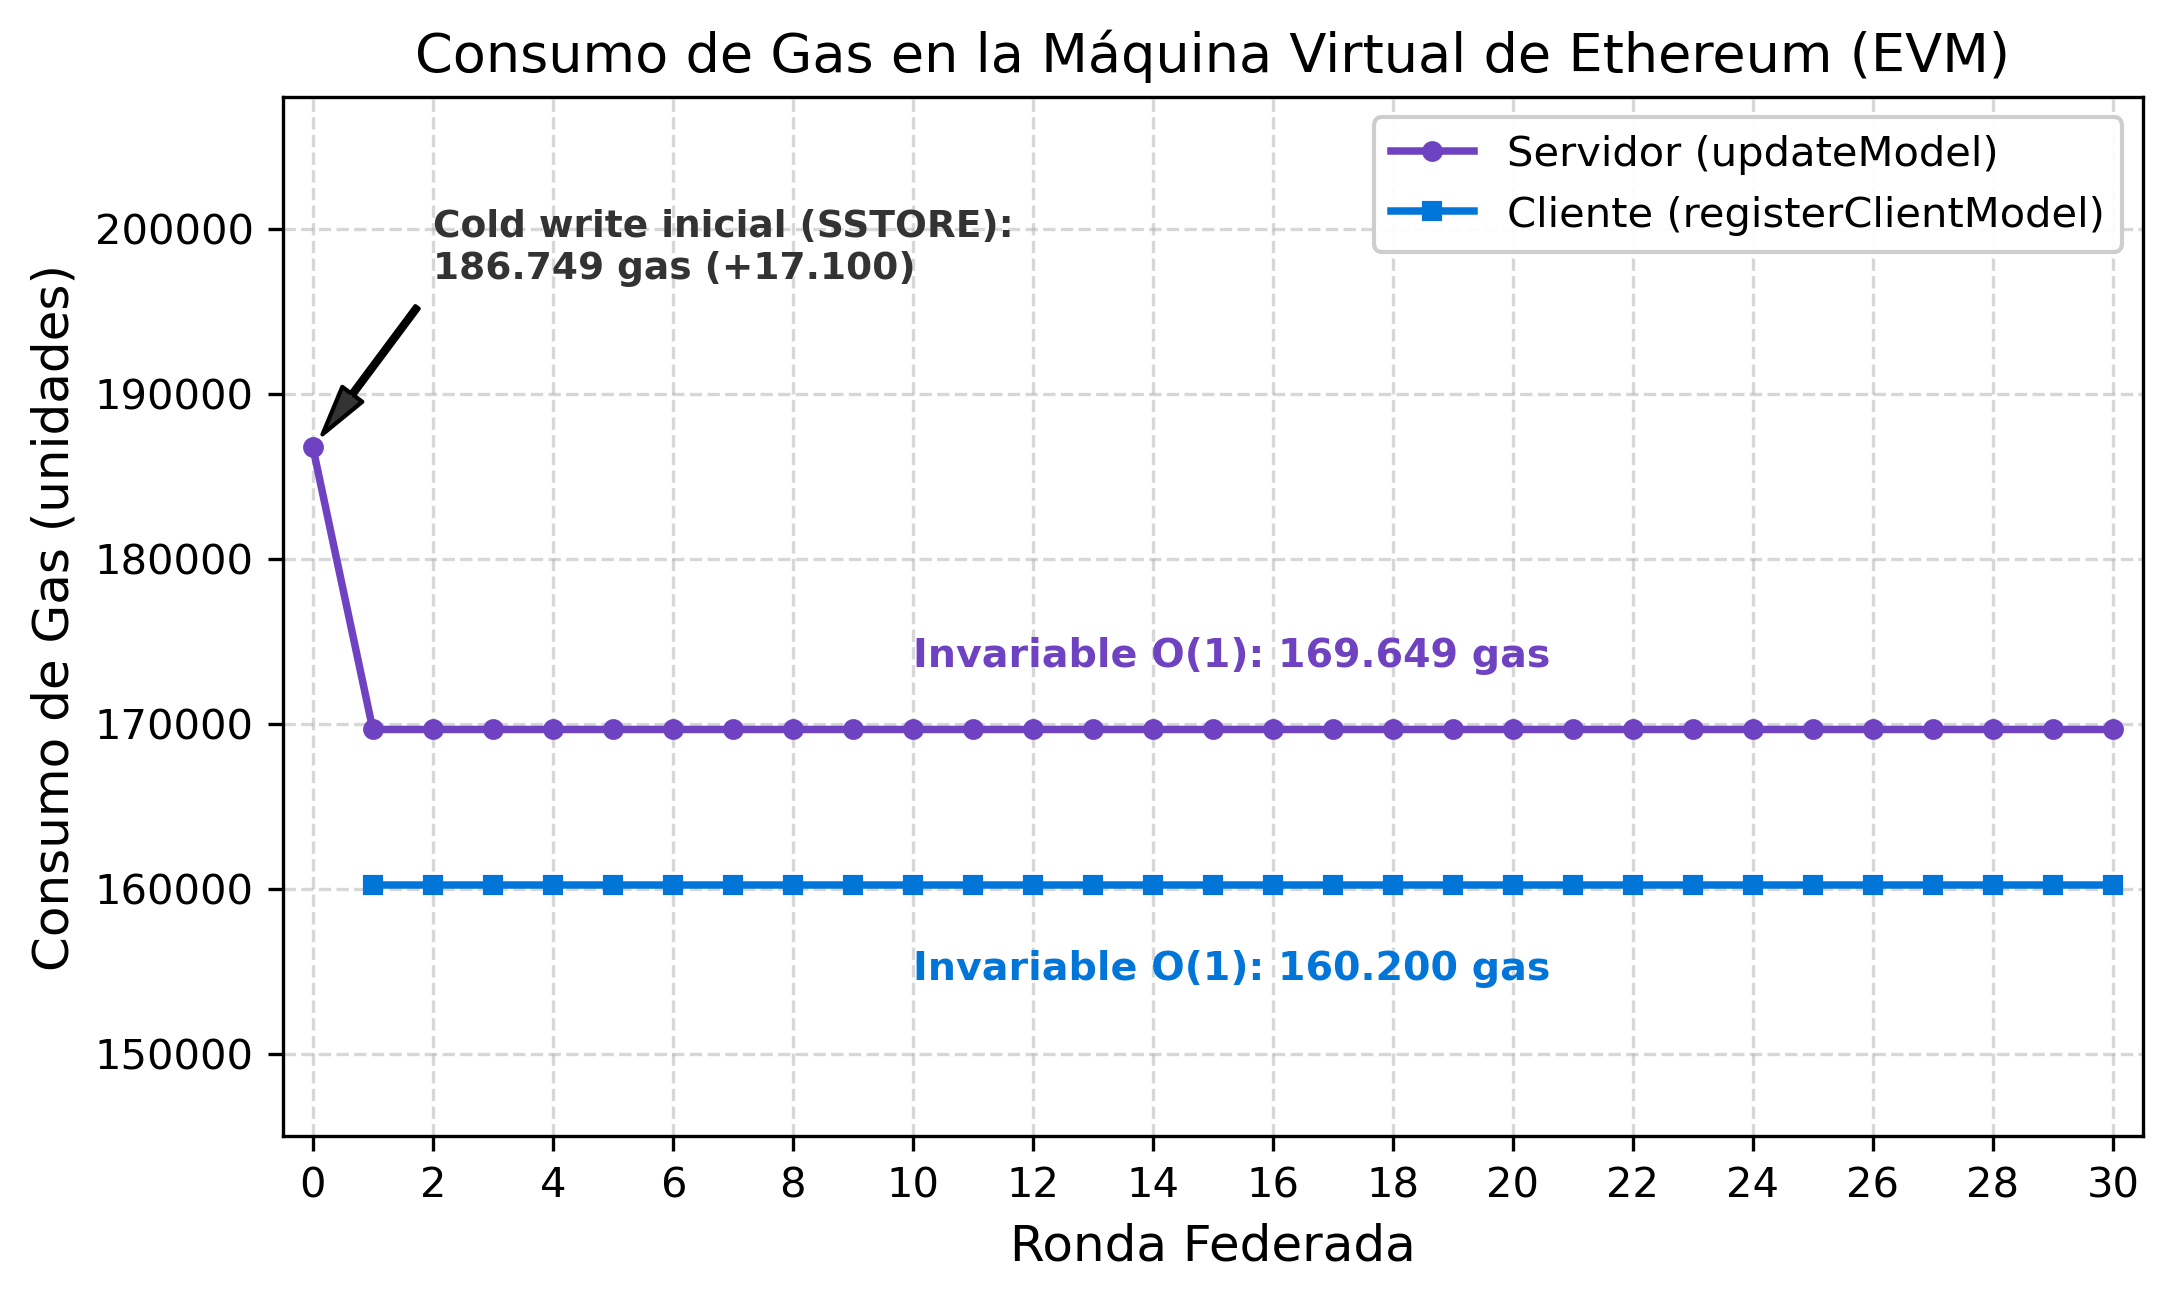
\includegraphics[width=0.70\columnwidth]{figuras/consumo_gas.png}
    \caption{Consumo de gas en la Máquina Virtual de Ethereum por tipo de transacción a lo largo de las 30 rondas.}
    \label{fig:consumo_gas}
\end{figure}

El perfil de consumo resulta rigurosamente constante en todas las iteraciones:
\begin{itemize}
    \item \texttt{registerClientModel}: exactamente \textbf{160.200 unidades de gas}.
    \item \texttt{updateModel}: exactamente \textbf{167.460 unidades de gas}.
\end{itemize}
Conviene destacar que este consumo refleja la versión definitiva del contrato inteligente \texttt{FLRegistry}: la inclusión del modificador de control de acceso \texttt{onlyServer} en \texttt{updateModel} introduce una comprobación de identidad en la EVM (\texttt{SLOAD} y salto condicional sobre \texttt{serverAddress}) que añade únicamente 100 unidades de gas (+0,06\% de sobrecoste respecto a una versión abierta sin control de acceso), manteniendo el coste acotado y plenamente predecible.
La única excepción observable corresponde a la ronda 0 del servidor, que demandó \textbf{184.560 unidades de gas}. Dicha discrepancia (+17.100 unidades) responde al coste de la instrucción \texttt{SSTORE} de la EVM al escribir por primera vez en posiciones de memoria previamente vacías (\textit{cold write}) y modificar el valor del flag booleano \texttt{hasModel}.

La invariabilidad del consumo valida formalmente el diseño desacoplado: al almacenar en el contrato únicamente cadenas de longitud uniforme (los identificadores CIDv0 de IPFS de 46 caracteres que encapsulan el multihash SHA-256 y metadatos acotados), el coste de gas se mantiene estable por transacción e independiente tanto del tamaño del modelo neuronal como del número acumulado de rondas, asegurando un consumo de recursos acotado y predecible en redes de consorcio.

\subsection{Auditoría de Inmutabilidad On-Chain y Trazabilidad Forense}
\label{subsec:auditoria_onchain}
Para verificar empíricamente la correspondencia unívoca entre los eventos del ciclo de vida de Flower y la persistencia inmutable en la cadena de bloques, la Tabla~\ref{tab:auditoria_transacciones} recoge una muestra representativa de los recibos de transacción (\textit{transaction receipts}) extraídos de la telemetría en tiempo de ejecución, correlacionada directamente con la visualización en el explorador de bloques de la red de consorcio (Figura~\ref{fig:auditoria_bloque}).

\begin{table}[H]
\centering
\caption{Muestra de trazabilidad y auditoría forense on-chain.}
\label{tab:auditoria_transacciones}
\resizebox{\columnwidth}{!}{%
\begin{tabular}{@{}cccccc@{}}
\toprule
\textbf{Bloque} & \textbf{Entidad} & \textbf{Evento / Método} & \textbf{Dirección Emisora} & \textbf{Prefijo Tx Hash} & \textbf{Gas EVM} \\
\midrule
8 & Servidor & Despliegue \texttt{FLRegistry} & \texttt{0xfe3b557e...} & \texttt{0x939eb46c...} & 1.999.000 \\
13 & Servidor & \texttt{updateModel} & \texttt{0xfe3b557e...} & \texttt{0xa18e3bb4...} & 167.460 \\
14 & Cliente 2 & \texttt{registerClientModel} & \texttt{0x62730609...} & \texttt{0xc1c7402f...} & 160.200 \\
\midrule
765 & Servidor & \texttt{updateModel} (Ronda 23) & \texttt{0xfe3b557e...} & \texttt{0x4ceabb7a...} & 167.460 \\
783 & Servidor & \texttt{updateModel} (Ronda 24) & \texttt{0xfe3b557e...} & \texttt{0xb9cb75f5...} & 167.460 \\
801 & Servidor & \texttt{updateModel} (Ronda 25) & \texttt{0xfe3b557e...} & \texttt{0xdf69295f...} & 167.460 \\
\bottomrule
\end{tabular}%
}
\end{table}

\begin{figure}[H]
    \centering
    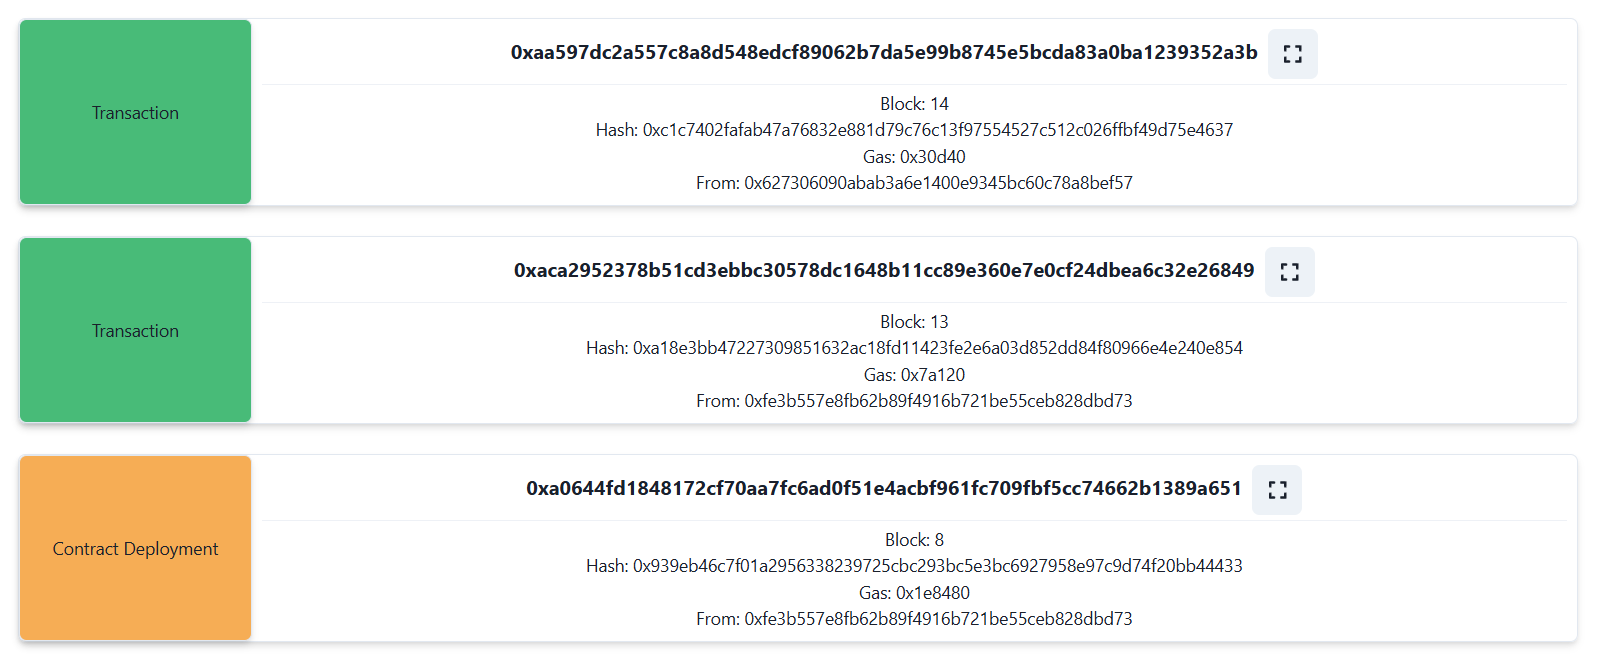
\includegraphics[width=0.96\columnwidth]{figuras/bloque_contrato.png}
    \caption{Auditoría de inmutabilidad on-chain: visualización en el explorador Besu del despliegue del contrato \texttt{FLRegistry} (Bloque~8) por el servidor (\texttt{0xfe3b55...}) junto a transacciones operativas 13 y 14.}
    \label{fig:auditoria_bloque}
\end{figure}

Cada identificador de bloque y hash criptográfico actúa como prueba forense no repudiable, confirmando la viabilidad de la arquitectura para auditorías regulatorias en sistemas vehiculares y de misión crítica.

% !TeX root = ../main.tex
\section{Conclusiones y Trabajo Futuro}
\label{sec:conclusiones}

En este artículo se ha presentado, implementado y validado experimentalmente un marco integral orientado a proporcionar trazabilidad, integridad y auditoría criptográfica en sistemas de Aprendizaje Federado, combinando una red Blockchain permisionada (Hyperledger Besu) con almacenamiento direccionable fuera de cadena (IPFS) y el framework Flower.

\subsection{Conclusiones Principales}
Los resultados obtenidos permiten extraer las siguientes conclusiones clave:
\begin{itemize}
    \item \textbf{Viabilidad técnica y sobrecoste temporal asumible}: La integración de la capa de trazabilidad en un despliegue distribuido en red introduce una sobrecarga temporal de tan solo el \textbf{9,5\%} (un incremento mediano de 6,34~segundos por ronda federada, pasando de 66,62~s a 72,96~s). Este sobrecoste responde afirmativamente al dilema de rendimiento vs. seguridad, demostrando que la auditabilidad de extremo a extremo es plenamente viable en sistemas de IA distribuida sin degradar la cadencia operativa.
    \item \textbf{Eficacia y rapidez de la doble verificación cruzada}: El diseño propuesto erradica la dependencia de un servidor central como punto único de confianza. Mediante el cotejo automático de CIDs de IPFS frente a los registros inmutables on-chain, los clientes quedan protegidos frente a modelos globales corruptos (abortando la ronda en $0{,}074$~s), mientras que el agregador descarta de inmediato contribuciones disidentes no firmadas (en $0{,}044$~s), alcanzando una tasa de detección del 100\% frente a los vectores de adulteración e inyección evaluados con tiempos de reacción inferiores a la décima de segundo.
    \item \textbf{Eficiencia y predictibilidad on-chain}: El desacoplamiento arquitectónico mediante IPFS asegura un coste de gas estable y predecible por transacción (160.200 gas para clientes y 167.460 gas para el servidor), evitando cualquier saturación del estado de la EVM con total independencia del tamaño de los pesos del modelo convolucional.
    \item \textbf{Escalabilidad del consenso BFT}: Incrementar los nodos validadores de 4 a 7 (duplicando la tolerancia a fallos bizantinos de $f=1$ a $f=2$) apenas eleva la latencia de confirmación de transacciones en $0{,}10$~segundos (100~ms) y la mediana de ronda en tan solo $0{,}39$~s, quedando este incremento absorbido de forma imperceptible dentro del cómputo de gradientes local.
\end{itemize}

\subsection{Limitaciones y Trabajo Futuro}
Como líneas de desarrollo futuro que amplían el alcance de este trabajo, se plantean:
\begin{enumerate}
    \item \textbf{Optimización y regularización del modelo de IA}: Dado que la meta primordial de este artículo consistió en evaluar la infraestructura y extraer métricas cuantitativas del sistema FL-Blockchain, la optimización fina de la red neuronal quedó fuera del alcance primario. Como línea futura se contempla incorporar criterios de parada temprana (\textit{early stopping}), técnicas de regularización (Dropout, normalización de batches) y arquitecturas convolucionales avanzadas para maximizar la generalización.
    \item \textbf{Mecanismos de reputación y penalización on-chain}: Explotar el historial inmutable de contribuciones para articular algoritmos de puntuación de clientes o penalización (\textit{slashing}) económica/lógica de nodos maliciosos recurrentes.
    \item \textbf{Agregación bizantina avanzada}: Complementar el esquema con estrategias de agregación robustas frente a envenenamiento no evidente (como Krum~\cite{blanchard2017byzantine} o medias recortadas) coordinadas desde el propio contrato.
    \item \textbf{Entornos no-IID y despliegue vehicular V2X}: Evaluar la robustez del framework bajo distribuciones de datos altamente heterogéneas y desplegar nodos en hardware embarcado (\textit{edge computing}, como NVIDIA Jetson) con conectividad celular 5G/V2X.
    \item \textbf{Gestión criptográfica de claves}: Sustituir el esquema de cuentas actual por módulos de seguridad de hardware (HSM) o almacenes seguros de secretos tipo Key Vault para un despliegue conforme a estándares industriales.
    \item \textbf{Control de acceso on-chain y gobernanza descentralizada}: Incorporar modificadores formales de control de acceso en el Smart Contract (\texttt{onlyServer} o esquemas de consenso multifirma y gobernanza basada en roles RBAC) para restringir directamente en el bytecode de la EVM la invocación de \texttt{updateModel}, reforzando la seguridad en despliegues con múltiples servidores agregadores o federaciones abiertas.
\end{enumerate}
En síntesis, la arquitectura validada demuestra que la convergencia entre Blockchain y Aprendizaje Federado no solo es factible, sino que establece una base metodológica y arquitectónica viable para el despliegue auditable y confiable de inteligencia artificial en entornos críticos y cooperativos.



\bibliographystyle{ieeepes}
\bibliography{bibliografia}

\begin{IEEEbiography}[{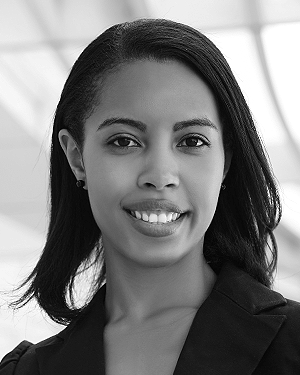
\includegraphics[width=1in,height=1.25in,clip,keepaspectratio]{a1.png}}]{David Piotr Znojek}
% Biografía pendiente de añadir
\end{IEEEbiography}

\begin{IEEEbiography}[{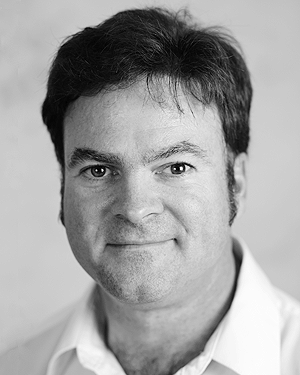
\includegraphics[width=1in,height=1.25in,clip,keepaspectratio]{a2.png}}]{Francisco A. Pujol}
% Biografía pendiente de añadir
\end{IEEEbiography}

\EOD

\end{document}
